% *======================================================================*
%  Cactus Thorn template for ThornGuide documentation
%  Author: Ian Kelley
%  Date: Sun Jun 02, 2002
%  $Header$
%
%  Thorn documentation in the latex file doc/documentation.tex
%  will be included in ThornGuides built with the Cactus make system.
%  The scripts employed by the make system automatically include
%  pages about variables, parameters and scheduling parsed from the
%  relevant thorn CCL files.
%
%  This template contains guidelines which help to assure that your
%  documentation will be correctly added to ThornGuides. More
%  information is available in the Cactus UsersGuide.
%
%  Guidelines:
%   - Do not change anything before the line
%       % START CACTUS THORNGUIDE",
%     except for filling in the title, author, date, etc. fields.
%        - Each of these fields should only be on ONE line.
%        - Author names should be separated with a \\ or a comma.
%   - You can define your own macros, but they must appear after
%     the START CACTUS THORNGUIDE line, and must not redefine standard
%     latex commands.
%   - To avoid name clashes with other thorns, 'labels', 'citations',
%     'references', and 'image' names should conform to the following
%     convention:
%       ARRANGEMENT_THORN_LABEL
%     For example, an image wave.eps in the arrangement CactusWave and
%     thorn WaveToyC should be renamed to CactusWave_WaveToyC_wave.eps
%   - Graphics should only be included using the graphicx package.
%     More specifically, with the "\includegraphics" command.  Do
%     not specify any graphic file extensions in your .tex file. This
%     will allow us to create a PDF version of the ThornGuide
%     via pdflatex.
%   - References should be included with the latex "\bibitem" command.
%   - Use \begin{abstract}...\end{abstract} instead of \abstract{...}
%   - Do not use \appendix, instead include any appendices you need as
%     standard sections.
%   - For the benefit of our Perl scripts, and for future extensions,
%     please use simple latex.
%
% *======================================================================*
%
% Example of including a graphic image:
%    \begin{figure}[ht]
% 	\begin{center}
%    	   \includegraphics[width=6cm]{MyArrangement_MyThorn_MyFigure}
% 	\end{center}
% 	\caption{Illustration of this and that}
% 	\label{MyArrangement_MyThorn_MyLabel}
%    \end{figure}
%
% Example of using a label:
%   \label{MyArrangement_MyThorn_MyLabel}
%
% Example of a citation:
%    \cite{MyArrangement_MyThorn_Author99}
%
% Example of including a reference
%   \bibitem{MyArrangement_MyThorn_Author99}
%   {J. Author, {\em The Title of the Book, Journal, or periodical}, 1 (1999),
%   1--16. {\tt http://www.nowhere.com/}}
%
% *======================================================================*

% If you are using CVS use this line to give version information
% $Header$

\documentclass{article}

% Use the Cactus ThornGuide style file
% (Automatically used from Cactus distribution, if you have a
%  thorn without the Cactus Flesh download this from the Cactus
%  homepage at www.cactuscode.org)
\usepackage{../../../../doc/latex/cactus}
\usepackage{listings}
\usepackage{graphics}
\usepackage{amsmath}

\usepackage[svgnames]{xcolor}
\usepackage{hyperref}
\hypersetup{colorlinks=true,urlcolor=Blue,linkcolor=Blue,citecolor=CornflowerBlue,naturalnames=true,hypertexnames=true}

\usepackage{tabularx}

% Code listing boxes
\lstset{
    language=C++,
    breaklines=true,
    basicstyle=\tt,
    keywordstyle=\color{blue},
    identifierstyle=\color{magenta},
    frame=single,
    numbers=left,
    stepnumber=1,
    showstringspaces=false,
}

\begin{document}

% The author of the documentation
\author{
    Erik Schnetter \textless eschnetter@perimeterinstitute.ca\textgreater \\
    Lucas Timotheo Sanches \textless lucas.t.s.carneiro@gmail.com\textgreater \\
    Steven R. Brandt \textless sbrandt@cct.lsu.edu\textgreater\\
}

% The title of the document (not necessarily the name of the Thorn)
\title{\texttt{CarpetX} User Manual}

% the date your document was last changed, if your document is in CVS,
% please use:
%    \date{$ $Date$ $}
% when using git instead record the commit ID:
%    \date{$ $Id$ $}
% and add this line to your repos' .gitattributes file:
% **.tex ident
\date{\today} % TODO: This should be replaced with the final date once we are done

\maketitle

% Do not delete next line
% START CACTUS THORNGUIDE

% Add all definitions used in this documentation here
\newcommand{\CarpetX}{\texttt{CarpetX}}
\newcommand{\Cactus}{\texttt{Cactus}}
\newcommand{\AMReX}{\texttt{AMReX}}
\newcommand{\ETK}{\texttt{Einstein Toolkit}}
\newcommand{\todo}[1]{\textcolor{red}{TODO: #1}}

\begin{figure*}[ht]
    \begin{center}
        
\includegraphics[width=6cm]{logo.png}
    \end{center}
    \label{fig:logo}
\end{figure*}

\newpage

% Add an abstract for this thorn's documentation
\begin{abstract}

\CarpetX\space is a \href{https://www.cactuscode.org/index.html}{\Cactus} driver thorn based on \href{https://amrex-codes.github.io/}{\AMReX}, a software framework for block-structured AMR (adaptive mesh refinement). \CarpetX\space is intended for the \href{https://einsteintoolkit.org/}{\ETK}.

Driver thorns are special modules that provide distributed data structures, refine meshes, perform memory allocation, and interfaces to parallel computing hardware and software. In short, they provide all the low-level basic infrastructure needed for any scientific simulation.

\end{abstract}

\newpage

\tableofcontents

\newpage

%%%%%%%%%%%%%%%%%%%%%%%%%%%%%%%%%%%%%%%%%%%%%%%%%%%%%%%%%%%%
\section{Introduction}
\label{sec:intro}

\todo{We should have some words explaining what \CarpetX\space is.}

%%%%%%%%%%%%%%%%%%%%%%%%%%%%%%%%%%%%%%%%%%%%%%%%%%%%%%%%%%%%
\section{Building and using standard images}
\label{sec:std_imgs}

There are a few standard images for CarpetX.

There are a set of them in the \texttt{docker} directory of \CarpetX's main \href{https://github.com/eschnett/CarpetX}{GitHub repository}. These build the various packages that \CarpetX\space depends on mostly by hand. This is probably the more official set of images.

Another is build from this \href{https://github.com/stevenrbrandt/carpetx-install}{Dockerfile}. This image is based on \href{https://github.com/spack/spack}{Spack}, a flexible, python-based system for installing packages. This image contains optionlist files for Cactus in \texttt{/usr/cactus/local-cpu.cfg} and \texttt{/usr/local-gpu.cfg}. This image also contains two versions of the hpctoolkit tool, one that is cuda-enabled and one that is not. This rather beefy image is nearly 40GB in size, but it provides you with a complete set of tools for building and running CarpetX, Cactus, and the various development projects taking place within that framework. The image is maintained at \texttt{docker.io/stevenrbrandt/etworkshop}.

If you are running on a cluster with Singularity installed, you can compile the image as follows:

\begin{lstlisting}
singularity build -F /work/sbrandt/images/etworkshop.simg \
    docker://stevenrbrandt/etworkshop
\end{lstlisting}

You can run the image using something like the following:
\begin{lstlisting}
srun singularity exec --nv \
     --bind /var/spool --bind /work \
     --bind /etc/ssh/ssh_known_hosts \
     exec /work/sbrandt/images/etworkshop.simg cactus_sim my_parfile.par
\end{lstlisting}

Whether you choose to use one of the above images, or create an installation based on what you find in the dockerfiles for the above images, we wish you luck in your compiling and running efforts.

%%%%%%%%%%%%%%%%%%%%%%%%%%%%%%%%%%%%%%%%%%%%%%%%%%%%%%%%%%%%
\section{CCL file settings and macros}
\label{sec:ccl_files}
CCL files are used to define cactus thorns and customize its behavior. In this section, we shall discuss the additions that \CarpetX\space brigs to these files, but we shall not teach users how to write them from scratch. In order to learn more, refer to Sec.~C of the \Cactus\space user guide provided in the \texttt{doc} folder of all distributions.

Users may need to require certain thorns explicitly in \texttt{configuration.ccl} files when using \CarpetX\space APIs or schedule functions at specific bins provided by thorns in the \CarpetX\space arrangement. These thorn-specific additions are documented in the thorn's section of this text.

An important point to note is that \CarpetX\space strongly enforces read, write and location statement correctness at runtime and compile time as declared in \texttt{schedule.ccl} files. This means that one is not able to write to a variable declared as \texttt{READ}. \CarpetX\space also marks points in regions as valid or invalid and impedes user of reading from invalid data points. These extra measures help users prevent common memory and region access bugs. 

\subsection{Macros}

In their \texttt{C++} code, users should always use the \texttt{DECLARE\_CCTK\_ARGUMENTSX\_<scheduled function name>} macro to ensure that only the objects declared in the function's schedule block in \texttt{schedule.ccl} are brought into scope, as well as other objects necessary for working with \CarpetX.

 \subsection{Centering}

The centering of a grid function is declared via \texttt{CENTERING={<centering-code>}}, where \texttt{<centering-code>} is a three-letter code containing any combination of either \texttt{c} or \texttt{v}, representing cell centering and vertex centering, respectively in \texttt{interface.ccl} files. For example, to declare a group of variables as being cell centered, one would use
%
\begin{lstlisting}
  CCTK_<type> <group-name> CENTERING={ccc}
  {
    ...
  } "A group of variables"
\end{lstlisting}

Similarly, for a vertex centered group one would use
%
\begin{lstlisting}
  CCTK_<type> <group-name> CENTERING={vvv}
  {
    ...
  } "A group of variables"
\end{lstlisting}

Note that it is possible to mix centering indexes. For example, to have a quantity centered at faces in the x direction, one would write
%
\begin{lstlisting}
  CCTK_<type> <group-name> CENTERING={cvv}
  {
    ...
  } "A group of variables"
\end{lstlisting}

Not also that if no \texttt{CENTERING} is specified, \CarpetX\space assumes that the variable group is vertex centered in all directions.

Finally, it is very important to match the centering description in interface files with the description passed to loop API template arguments. See Sec.~\ref{sec:loops} for details.

\subsection{Tags}
\label{sec:tags}

Tags are declared in interface statements (in \texttt{interface.ccl}) with the \texttt{TAGS=<tags>} syntax. The \texttt{<tags>} declaration consists of a single quote string (marked by \texttt{'}) with space separated key-value pars of the form \texttt{key="value"}. For example, a tagged interface declaration will be similar to the following
%
\begin{lstlisting}[language=bash]
  CCTK_<type> <group-name> TAGS='key_1="key1" key_2="key2" ...'
  {
    ...
  } "A group of variables"
\end{lstlisting}

We will now list the tags supported by \CarpetX\space and describe their usage.

\subsubsection{\texttt{rhs}}

Marks a group of grid variables as the RHS (right-hand side) of a system. \texttt{ODESolvers} uses this information to perform time steps and update a state vector (See Sec.~\ref{sec:odesolvers} for more information). For example, in
%
\begin{lstlisting}[language=bash]
  CCTK_<type> state_vector TAGS='rhs="right_hand_side"'
  {
    ...
  } "A group of variables representing the PDE system state"

  CCTK_<type> right_hand_side
  {
    ...
  } "A group of variables representing the PDE RHS"
\end{lstlisting}
%
the \texttt{rhs="right\_hand\_side"} tag indicates that the group named \texttt{state\_vector} has a corresponding RHS group named \texttt{right\_hand\_side}.

\begin{lstlisting}[language=bash]
  CCTK_<type> state_vector TAGS='rhs="right_hand_side"'
  {
    ...
  } "A group of variables representing the PDE system state"
\end{lstlisting}

\subsubsection{\texttt{dependents}}

Indicates that the groups of variables contained on this tag must be marked as invalid if there are any changes to the group being declared. For example, in
%
\begin{lstlisting}[language=bash]
  CCTK_<type> parent_group TAGS='dependents="child1 child2"'
  {
    ...
  } "A group of real variables"
\end{lstlisting}
%
the tag \texttt{dependents="child1 child2"} indicates that \texttt{parent\_group} has two dependent groups, \texttt{child1} and \texttt{child2}. Whenever \CarpetX\space writes to variables in \texttt{parent\_group}, variables in \texttt{child1} and \texttt{child2} are marked as invalid and cannot be read from unless written to again.

\subsubsection{\texttt{checkpoint}}

Indicates that a variable group must be saved as a simulation checkpoint. \Cactus\space and \CarpetX\space can then later recover the saved checkpoint variables and restore the simulation state to continue evolution from there. Usually, only state vectors are checkpointed (See Chap. A3 of the \Cactus user manual for further details). For example, in
%
\begin{lstlisting}[language=bash]
  CCTK_<type> state_vector TAGS='checkpoint="yes"'
  {
    ...
  } "A group of real variables describing the simulation state"

  CCTK_<type> right_hand_side TAGS='checkpoint="no"'
  {
    ...
  } "A group of real variables describing the simulation RHS"
\end{lstlisting}
%
the simulation state, represented by the \texttt{state\_vector} group is checkpointed, while the \texttt{right\_hand\_side} group is not.

The parameters \texttt{CarpetX::checkpoint\_method} and \texttt{CarpetX::recover\_method} control \CarpetX's behavior during variable checkpointing and recovery, respectively. Both parameters accept the same keyword values, described in Tab.~\ref{tab:checkpoint_recovery}

\begin{table}[hb]
  \centering
  \begin{tabular}{cc}
  Setting value    & Effect                                                         \\ \hline\hline
  \texttt{error}   & Abort with error instead of checkpointing/recovering (default) \\
  \texttt{openpmd} & Uses \texttt{openpmd} formatted files for writing checkpoints  \\
  \texttt{silo}    & Uses \texttt{silo} files for writing checkpoints               \\ \hline\hline
  \end{tabular}
  \caption{Possible values for \texttt{CarpetX::checkpoint\_method} and \texttt{CarpetX::recover\_method} and their effects on checkpointing and recovery.}
  \label{tab:checkpoint_recovery}
\end{table}

\todo{Using \texttt{TerminationTrigger} to control checkpointing does not work yet.}

To control when a checkpoint is to be produced, users first need to set the flash parameter \texttt{Cactus::terminate}, which controls under which conditions a simulation is to be terminated (see Sec.~D5.2 of the \Cactus\space user guide for further details on possible values for this parameter). After that, they can control various aspects of the checkpoint files produced, such as name and checkpoint file production on termination by setting parameters in the \texttt{IO} thorn. This is an infrastructure thorn that is always active and communicates its settings to \CarpetX, which is effectively responsible for writing data to disk. To see all available parameters that can be set in \texttt{IO}, read the file \texttt{Cactus/repos/cactusbase/IOUtil/param.ccl} lines 137-205. These parameters are well documented in this file. 

Additionally, it is \textit{imperative} to set the flash's presync mode to \texttt{"presync-only"} by adding \texttt{Cactus::presync\_mode = "presync-only"} to the simulation's parameter file. Failure to do so will cause the recovered checkpoints to be valid only on the interior and not on ghosts and boundaries (See Sec.~D5.2 of the \Cactus\space user guide for more information on presync modes).

As an example, we present an excerpt of a parameter file for a simulation that ends after simulation time reaches $t=100$, but we allow \Cactus\space running for only 1 minute of wall time. For the physical system being simulated, such execution time is not enough for the system to reach $t=100$, thus the execution of \Cactus\space will be terminated before the system is completely evolved. We would like to be able to recover from the last iteration performed by the system in subsequent executions of \Cactus. To do that, we will configure the \texttt{IO} thorn to produce checkpoint files upon \Cactus\space termination.

\begin{lstlisting}[language=bash]
  # Required in order to recover successfully
  Cactus::presync_mode = "presync-only"

  # The type of checkpoint and recovery files that should be used
  CarpetX::checkpoint_method = "openpmd"
  CarpetX::recover_method    = "openpmd"

  # Schedule termination of the simulation for 1 minute of wall time
  Cactus::terminate       = "runtime"
  Cactus::cctk_final_time = 100.0
  Cactus::max_runtime     = 1.0

  # Configure IO to produce checkpoint files before terminating
  IO::checkpoint_ID           = no
  IO::recover                 = "autoprobe"
  IO::out_proc_every          = 2
  IO::checkpoint_on_terminate = yes
  IO::checkpoint_dir          = "../checkpoints"
  IO::recover_dir             = "../checkpoints"
  IO::abort_on_io_errors      = yes
\end{lstlisting}

\subsection{\texttt{parity}}
The \texttt{parity} tag controls a tensor's reflection symmetries about the \texttt{x}, \texttt{y} and \texttt{z} axes. There are 3 parities for each tensor component, representing the symmetries about the 3 spatial axes.

For example, a scalar, has \texttt{parities=\{+1 +1 +1\}}, which indicates that no sign changes take place when the quantity is reflected around the axes. If no \texttt{parities} tag is present in a variable group declaration, it is assumed to be a scalar and \texttt{parities=\{+1 +1 +1\}} is implicitly assumed. For a vector, the \texttt{parities=\{-1 +1 +1\hspace{15pt}+1 -1 +1\hspace{15pt}+1 +1 -1\}} tag indicates in the first triad of numbers that the vector's \texttt{x} component changes sign while being reflected in the \texttt{x} direction, the second triad indicates that the \texttt{y} component changes sign while reflected in the \texttt{y} direction and the third triad indicates that the \texttt{z} component changes sign while being reflected in the \texttt{z} direction. As an example, let us look at the parities of the energy momentum tensor in general relativity as declared in the \texttt{interface.ccl} file of the \texttt{TmunuBaseX} thorn included in \CarpetX\space: 
%
\begin{lstlisting}[language=bash]
# The T_{tt} component represents the energy density and
# is stored as a scalar. The parities={+1 +1 +1} tag is implicit.
CCTK_REAL eTtt TAGS='checkpoint="no"' TYPE=gf "T_00"

# The T_{ti} components of the tensor are a vector of three entries.
# Each component changes sign when reflected on their respective axes.
CCTK_REAL eTti TAGS='parities={-1 +1 +1    +1 -1 +1    +1 +1 -1} checkpoint="no"' TYPE=gf
{ 
    eTtx eTty eTtz
} "T_0i"

# The T_{ij} components form a rank 2 tensor of 3 spatial dimensions.
# Each index triplet represents a component in the tensor.
CCTK_REAL eTij TAGS='parities={+1 +1 +1    -1 -1 +1    -1 +1 -1    +1 +1 +1    +1 -1 -1    +1 +1 +1} checkpoint="no"' TYPE=gf
{
    eTxx eTxy eTxz eTyy eTyz eTzz
} "T_ij"

# The parities tag on this tensor indicates that:
# * The xx component does not change sign.
# * The xy component changes sign while reflecting on either x or y.
# * The xz component changes sign while reflecting on either x or z.
# * The yy component does not change sign.
# * The yz component changes sign while reflecting on either y or z.
# * The zz component does not change sign.
\end{lstlisting}

%%%%%%%%%%%%%%%%%%%%%%%%%%%%%%%%%%%%%%%%%%%%%%%%%%%%%%%%%%%%
\section{Creating grids}
\label{sec:grids}

In this section, we will describe \CarpetX's parameters used for describing the simulation domain. Currently, \CarpetX\space supports only Cartesian grids. To control the grid's extents, users must utilize parameters described in Tab.~\ref{tab:grid_sizes}. To control the number of cells in each direction, users must set the parameters described in Tab.~\ref{tab:num_cells}. Finally, to control the number of ghost zones in the grid, users must set the parameters described in Tab.~\ref{tab:ghost_sizes}. It is important to note that the size of all ghost zones can be set at once via \texttt{ghost\_size} parameter or via the \texttt{ghost\_size\_xyz} family of parameters if \texttt{ghost\_size} is set to $-1$

\begin{table}[ht]
  \centering
  \begin{tabular}{ccc}
  Parameter     & Description                                    & Default value \\\hline\hline
  \texttt{xmin} & Minimum value of the grid in the $x$ direction & $-1.0$        \\
  \texttt{xmax} & Maximum value of the grid in the $x$ direction & $1.0$         \\
  \texttt{ymin} & Minimum value of the grid in the $y$ direction & $-1.0$        \\
  \texttt{ymax} & Maximum value of the grid in the $y$ direction & $1.0$         \\
  \texttt{zmin} & Minimum value of the grid in the $z$ direction & $-1.0$        \\
  \texttt{zmax} & Maximum value of the grid in the $z$ direction & $1.0$         \\\hline\hline
  \end{tabular}
  \caption{Parameters controlling grid extents in \CarpetX.}
  \label{tab:grid_sizes}
\end{table}

\begin{table}[ht]
  \centering
  \begin{tabular}{ccc}
  Parameter          & Description                               & Default value \\\hline\hline
  \texttt{ncells\_x} & Number of grid cells in the $x$ direction & $128$         \\
  \texttt{ncells\_y} & Number of grid cells in the $y$ direction & $128$         \\
  \texttt{ncells\_z} & Number of grid cells in the $z$ direction & $128$         \\\hline\hline
  \end{tabular}
  \caption{Parameters controlling grid resolutions in \CarpetX.}
  \label{tab:num_cells}
\end{table}

\begin{table}[ht]
  \centering
  \begin{tabular}{ccc}
  Parameter             & Description                                & Default value \\\hline\hline
  \texttt{ghost\_size}    & Number of grid cells in all directions.    & $-1$          \\
  \texttt{ghost\_size\_x} & Number of ghost zones in the $x$ direction & $1$           \\
  \texttt{ghost\_size\_y} & Number of ghost zones in the $y$ direction & $1$           \\
  \texttt{ghost\_size\_z} & Number of ghost zones in the $z$ direction & $1$           \\\hline\hline
  \end{tabular}
  \caption{Parameters controlling the number of grid ghost zones in \CarpetX.}
  \label{tab:ghost_sizes}
\end{table}

%%%%%%%%%%%%%%%%%%%%%%%%%%%%%%%%%%%%%%%%%%%%%%%%%%%%%%%%%%%%
\section{Loops over grid elements}
\label{sec:loops}

In \CarpetX\space loops over grid elements are not written explicitly. Operations that are to be executed for every grid element (cells, edges or points) are specified via \texttt{C++} \href{https://en.cppreference.com/w/cpp/language/lambda}{\textit{lambda functions}}, also known as closures or anonymous functions.

These objects behave like regular \texttt{C++} functions, but can be defined \textit{inline}, that is, on the body of a function or as an argument to another function.

An important concept to grasp with lambda function is \textit{captures}. If a lambda (let us call this the child function) is defined in the body of an outer function (let us call this the parent function), the child can access variables defined in the parent function, provided that these variables are \textit{captured}. The two most relevant modes of capture while using \CarpetX\space are \textit{capture by reference} (denoted with the \texttt{\&} sign in the square brackets denoting the start of the lambda) and \textit{capture by value} (denoted by an \texttt{=} sign inside the square brackets of the lambda declaration).

When running on GPUs, captures by value are \textit{required} and captures by reference are \textit{forbidden}. This is because data must be copied from host (CPU side) memory to device (GPU side) memory in order to be executed.

The API for writing loops in \CarpetX\space is provided by the \texttt{Loop} thorn. To use it, one must add
%
\begin{lstlisting}[language=Bash]
    REQUIRES Loop
\end{lstlisting}
%
to the thorn's \texttt{configuration.ccl} file and
%
\begin{lstlisting}[language=Bash]
    INHERITS: CarpetX   
    USES INCLUDE HEADER: loop_device.hxx
\end{lstlisting}
%
to the thorn's \texttt{interface.ccl} file. Furthermore, one must include the \texttt{Loop} API header file in all source files where the API is needed by adding
%
\begin{lstlisting}
    #include <loop_device.hxx>
\end{lstlisting}
%
to the beginning of the source file.

%%%%%%%%%%%%%%%%%%%%%%%%%%%%%%%%%%%%%%%%%%%%%%%%%%%%%%%%%%%%
\subsection{Loop regions}
\label{sec:loop_regions}

Before actually writing any code that iterates over grid elements, one must choose \textit{which} elements are to be iterated over. We shall refer to the set of points in the grid hierarchy that will be iterated over when a loop is executed as a \textit{Loop region}. The following regions are defined in the \texttt{Loop} API:

\begin{enumerate}
    \item All: This region refers to all points contained in the grid. Denoted in code by the \texttt{all} suffix.
    
    \item Interior: This region refers to the interior of the grid. Denoted in code by the \texttt{int} prefix.
    
    \item Outermost interior: This region refers to the outermost "boundary" points in the interior. They correspond to points that are shifted inwards by = cctk\_nghostzones[3] from those that CarpetX identifies as boundary points. From the perspective of CarpetX (or AMReX), these do not belong in the outer boundary, but rather the interior. This excludes ghost faces, but includes ghost edges/corners on non-ghost faces. Loop over faces first, then edges, then corners. Denoted in code by the \texttt{outermost\_int} suffix.
\end{enumerate}

\todo{Picture of grid regions}

%%%%%%%%%%%%%%%%%%%%%%%%%%%%%%%%%%%%%%%%%%%%%%%%%%%%%%%%%%%%
\subsection{Loop methods}
\label{sec:loop_methods}

Loop API functions are methods of the \texttt{GridDescBaseDevice} class which contain functions for looping over grid elements on the CPU or GPU, respectively. The macro \texttt{DECLARE\_CCTK\_ARGUMENTSX\_FUNCTION\_NAME} provides a variable called \texttt{grid}, which is an instance of either of these classes. The name of each looping method is formed according to
%
\begin{center}
    \texttt{loop\_} + \textless loop region\textgreater + [\_\texttt{device}]
\end{center}

For example, to loop over boundaries using the CPU one would call
%
\begin{lstlisting}
    grid.loop_bnd<...>(...);
\end{lstlisting}
%
To obtain a GPU equivalent version, one would simply append \texttt{\_device} to the function name. Thus, for example, to loop over the interior using a GPU, one would call 

\begin{lstlisting}
    grid.loop_int_device<...>(...);
\end{lstlisting}

Let us now look at the required parameter of loop methods. The typical signature is as follows

\begin{lstlisting}
  template <int CI, int CJ, int CK, ..., typename F>
  void loop_REG_PU(const vect<int, dim> &group_nghostzones, const F &f);
\end{lstlisting}

The template parameters meanings are as follows:

\begin{enumerate}
  \item \texttt{CI}: Centering index for the first grid direction. Must be set explicitly and be either 0 or 1. 0 means that this direction will be looped over grid vertices, while 1 means that it will be looped over cell centers.
  \item \texttt{CJ}: Centering index for the second grid direction. Must be set explicitly and be either 0 or 1. 0 means that this direction will be looped over grid vertices, while 1 means that it will be looped over cell centers.
  \item \texttt{CK}: Centering index for the third grid direction. Must be set explicitly and be either 0 or 1. 0 means that this direction will be looped over grid vertices, while 1 means that it will be looped over cell centers.
  \item \texttt{F}: The type signature of the lambda function passed to the loop. It is not required to be set explicitly and is automatically deduced by the compiler.
\end{enumerate}

Note that centering indexes can be mixed: setting the indices to $(1,0,0)$, for instance, creates loops over faces on the \texttt{x} direction. Function parameter meanings are as follows:

\begin{enumerate}
  \item \texttt{group\_nghostzones}: The number of ghost zones in each direction of the grid. This can be obtained by calling \texttt{grid.nghostzones}.
  \item \texttt{f}: The \texttt{C++} lambda to be executed on each step of the loop.
\end{enumerate}

%%%%%%%%%%%%%%%%%%%%%%%%%%%%%%%%%%%%%%%%%%%%%%%%%%%%%%%%%%%%
\subsection{Loop Lambdas}

We shall now discuss the syntax and the available elements of the lambda functions that are to be fed to the Loop methods described in Section \ref{sec:loop_methods}.

To start, let us be reminded of the general syntax of a lambda function in \texttt{C++}:

\begin{lstlisting}
  // append ; if assigning to a variable
  [capture_parameter] (argument_list) -> return_type { function_body }
\end{lstlisting}

When running on GPUs, the \texttt{capture\_parameter} field used should always be \texttt{=}, indicating pass by value (copy) rather than \texttt{\&}, indicating pass by reference. The \texttt{argument\_list} of the lambda should receive only one element of type \texttt{PointDesc} (which will be described on Sec.~\ref{sec:point_des}) and the lambda must return no value, which means that \texttt{return\_type} can be omitted altogether.

This means that a typical lambda passed to a loop method will have the form
%
\begin{lstlisting}
  [=] (const Loop::PointDesc &p) {
    // loop body
  }
\end{lstlisting}

In addition, users can specify inlining (a compile-time optimization where the function call is replaced by its body) by using the \texttt{CCTK\_ATTRIBUTE\_ALWAYS\_INLINE} macro and designate host or device availability via the \texttt{CCTK\_HOST} or \texttt{CCTK\_DEVICE} macros, respectively. These annotations are optional unless the compiler is unable to build a function due to an inability to automatically determine that it needs to be available for device usage, for example. However, when these annotations are desired, they must be placed in specific locations.

To mark a lambda for host usage, one would use:
%
\begin{lstlisting}
  [=] CCTK_HOST(const Loop::PointDesc &p) CCTK_ATTRIBUTE_ALWAYS_INLINE {
    // loop body
  }
\end{lstlisting}
%
For device usage, one would use:
%
\begin{lstlisting}
  [=] CCTK_DEVICE(const Loop::PointDesc &p) CCTK_ATTRIBUTE_ALWAYS_INLINE {
    // loop body
  }
\end{lstlisting}
%
For both host and device usage, one would use:
%
\begin{lstlisting}
  [=] CCTK_HOST CCTK_DEVICE(const Loop::PointDesc &p) CCTK_ATTRIBUTE_ALWAYS_INLINE {
    // loop body
  }
\end{lstlisting}

%%%%%%%%%%%%%%%%%%%%%%%%%%%%%%%%%%%%%%%%%%%%%%%%%%%%%%%%%%%%
\subsection{The \texttt{PointDesc} type and loop lambda body}
\label{sec:point_des}

The \texttt{PointDesc} type provides a complete description of the current grid element in the loop. The following members are the ones that are expected to be used more often:
%
\begin{enumerate}
  \item \texttt{I}: A 3-element array containing the grid point indices.
  \item \texttt{DI}: A 3-element array containing the direction unit vectors from the current grind point.
  \item \texttt{X}: A 3-element array containing the point's coordinates.
  \item \text{DX}: A 3-element array containing the point's grid spacing.
  \item {iter}: The current loop iteration.
  \item {BI}: A 3-element array containing the outward boundary normal if the current point is the outermost interior point or zero otherwise.
\end{enumerate}

In the body of a loop lambda, grid functions declared in the thorn's \texttt{interface.ccl} file are available as \texttt{GF3D2} objects, which are \texttt{C++} wrappers around native \Cactus\space grid functions. These objects are accessible by directly calling them as functions taking arrays of grid indices as input. Such indices, in turn can be obtained by directly accessing \texttt{PointDesc} members.

\subsection{Example: Computing a RHS with finite differences}

Let us now combine the elements describe thus far into a single example. Let us suppose that the following system of PDEs is implemented in \Cactus:

\begin{align}
  \partial_t u & = \rho \label{eq:toy_loop_0}\\
  \partial_t \rho & = \partial_x^2 u + \partial_y^2 u + \partial_z^2 u \label{eq:toy_loop_1}
\end{align}

Let us suppose that the grid functions \texttt{u} and \texttt{rho} where made available, while grid functions \texttt{u\_rhs} and \texttt{rho\_rhs} are their corresponding RHS storage variables. The function that computes the RHS of Eqs.~\eqref{eq:toy_loop_0}-\eqref{eq:toy_loop_1} can be written as

\begin{lstlisting}
extern "C" void LoopExample_RHS(CCTK_ARGUMENTS) {
  DECLARE_CCTK_ARGUMENTS_LoopExample_RHS;
  DECLARE_CCTK_PARAMETERS;

  // The grid variable is implicitly defined via the CCTK macros
  // A 0/1 in template parameters indicate that a grid is vertex/cell centered
  grid.loop_int<0, 0, 0>(
    grid.nghostzones,

    // The loop lambda
    [=] (const Loop::PointDesc &p) {
      using std::pow;

      const CCTK_REAL hx = p.DX[0] * p.dX[0];
      const CCTK_REAL hy = p.DX[1] * p.dX[1];
      const CCTK_REAL hz = p.DX[2] * p.dX[2];
      
      const CCTK_REAL dudx = u(p.I - p.DI[0]) - 2 * u(p.I) 
        + u(p.I + p.DI[0])/hx;

      const CCTK_REAL dudy = u(p.I - p.DI[1]) - 2 * u(p.I) 
        + u(p.I + p.DI[1])/hy;

      const CCTK_REAL dudz = u(p.I - p.DI[2]) - 2 * u(p.I) 
        + u(p.I + p.DI[2])/hz;

      u_rhs(p.I) = rho(p.I);
      rho_rhs(p.I) = ddu;

    } // Ending of the loop lambda
  ); // Ending of the loop_int call
}
\end{lstlisting}

\subsection{SIMD Vectorization of loops}

If the user's CPU supports SIMD instructions (see \href{https://en.wikipedia.org/wiki/Single_instruction,_multiple_data}{here} for details), \CarpetX\space is capable of vectorizing loops via the \texttt{Arith} thorn. To use it, users must add
%
\begin{lstlisting}[language=bash]
  USES INCLUDE HEADER: simd.hxx
  USES INCLUDE HEADER: vect.hxx
\end{lstlisting}
%
to the top of their \texttt{interface.ccl} files, in addition to the other required headers.

While writing SIMD vectorized code, one has to keep in mind that grid functions are not a collection of \texttt{CCTK\_REAL} values but a collection of \texttt{Arith::simd<CCTK\_REAL>} real values, which is itself a collection of \texttt{CCTK\_REAL} values. This becomes apparent when reading and writing to grid functions at a particular grid point. To see how these differences come about, let us study an example of initializing grid data using the SIMD API
%
\begin{lstlisting}
  extern "C" void SIMDExample_Initial(CCTK_ARGUMENTS) {
  DECLARE_CCTK_ARGUMENTSX_SIMDExample_Initial;
  DECLARE_CCTK_PARAMETERS;

  using real = CCTK_REAL;
  using vreal = Arith::simd<real>;
  
  // This is the compile time determined vector size supported by the underlying CPU architecture
  constexpr std::size_t vsize = std::tuple_size_v<vreal>;

  // After passing the centering indices, size of the SIMD vectors is passed as template arguments
  grid.loop_int_device<0, 0, 0, vsize>(
    grid.nghostzones,
    
    [=] (const Loop::PointDesc &p) {
      // p.x is a scalar, but must be turned into a vector
      const vreal x0 = p.x + Arith::iota<vreal>() * p.dx;
      const real y0 = p.y;
      const real z0 = p.z;
      
      // The initialization function takes its inputs as vectors
      vreal u0, rho0;
      initial_data(x0, y0, z0, u0, rho0);
      
      u.store(p.mask, p.I, u0);
      rho.store(p.mask, p.I, rho0);
    }
  );
}
\end{lstlisting}

In lines 5 and 6, we define aliases for the real scalar type \texttt{CCTK\_REAL} and its associated vector type \texttt{Arith::simd<real>}. Values assigned to grid functions need to be of this type. In line 9, the \texttt{vsize} variable stores the size of the SIMD vectors of the target CPU. The \texttt{constexpr} keyword ensures that this expression is evaluated at compile time. In line 12, we call a loop API function with the three centering indices, discussed in Sec.~\ref{sec:loop_methods}, plus the extra \texttt{vreal} parameter which informs the loop method call that the loops will be vectorized.

At this point, it is very important to realize that loops can only be vectorized along the \texttt{x} direction. This is so because in SIMD vectors, entries must be sequential and internally, \CarpetX stores 3D grid data as a flattened array and only the \texttt{x} direction is contiguous. Line 17 is responsible for the vectorization of the \texttt{x} direction. The \texttt{Arith::iota<vreal>()} instruction produces an array of contiguously increasing elements from 0 to \texttt{vsize} (not end inclusive) which then gets multiplied by \texttt{p.dx} and incremented by \texttt{p.dx}. As an illustrative example, let us suppose that $\texttt{vsize} = 4$. In this case, 
%
\begin{equation}
  \texttt{Arith::iota<vreal>()} = 
  \begin{pmatrix}
    0\\
    1\\
    2\\
    3
  \end{pmatrix}
  .
\end{equation}
%
The operation on line 17 becomes then
%
\begin{equation}
  \texttt{x0} = \texttt{p.x} +
  \begin{pmatrix}
    0\\
    1\\
    2\\
    3\\
  \end{pmatrix}
  \texttt{p.dx} =
  \begin{pmatrix}
    \texttt{p.x}\\
    \texttt{p.x} + \texttt{p.dx}\\
    \texttt{p.x} + 2 * \texttt{p.dx}\\
    \texttt{p.x} + 3 * \texttt{p.dx}\\
  \end{pmatrix}
\end{equation}

On lines 22 and 23, the \texttt{initial\_data} function gets called and uses the vectorized \texttt{x0} coordinates and scalar coordinates \texttt{y0} and \texttt{z0} to fill the vectorized initial data variables \texttt{u0} and \texttt{rho0} which then finally get assigned to their respective grid functions via the \texttt{assign} member on lines 25 and 26. The \texttt{initial\_data} is arbitrary and user defined, but note that \texttt{Arith} overloads arithmetic operators and trigonometric functions, so it is straightforward to write code that uses vectorized and scalar variables together. 

Let us now look at an example of writing derivatives and RHS functions with SIMD loops.

\begin{lstlisting}
  extern "C" void SIMDExample_RHS(CCTK_ARGUMENTS) {
  DECLARE_CCTK_ARGUMENTSX_SIMDExample_RHS;
  DECLARE_CCTK_PARAMETERS;

  using vreal = Arith::simd<CCTK_REAL>;
  constexpr std::size_t vsize = std::tuple_size_v<vreal>;

  grid.loop_int_device<0, 0, 0, vsize>(
    grid.nghostzones,
    
    [=] (const Loop::PointDesc &p) {
      using Arith::pow2;

      const auto d2udx2 = (u(p.mask, p.I - p.DI[0]) - 2 * u(p.mask, p.I) + u(p.mask, p.I + p.DI[0]) ) / pow2(p.DX[0]);
      
      const auto d2udy2 = (u(p.mask, p.I - p.DI[1]) - 2 * u(p.mask, p.I) + u(p.mask, p.I + p.DI[1]) ) / pow2(p.DX[1]);
      
      const auto d2udz2 = (u(p.mask, p.I - p.DI[2]) - 2 * u(p.mask, p.I) + u(p.mask, p.I + p.DI[2]) ) / pow2(p.DX[2]);

      const auto udot = rho(p.mask, p.I);
      const auto rhodot = ddu;

      u_rhs.store(p.mask, p.I, udot);
      rho_rhs.store(p.mask, p.I, rhodot);
    });
  }
\end{lstlisting}

As previously mentioned, \texttt{Arith} overloads arithmetic operators, which makes writing mathematical expressions in vectorized loops no different from their non-vectorized counterparts. This is exemplified in lines 14-18 where second derivatives are being taken via finite differences approximations. Note once again in line 8 the presence of an extra template argument indicating the CPU's vector sizes, the extra \texttt{p.mask} argument being passed on all invocations of grid functions and the use of the \texttt{store} method to assign computed values to the RHS grid functions.

\todo{Document fused SIMD operations}

%%%%%%%%%%%%%%%%%%%%%%%%%%%%%%%%%%%%%%%%%%%%%%%%%%%%%%%%%%%%
\section{Time integration using \texttt{ODESolvers}}
\label{sec:odesolvers}

In \CarpetX, time integration of PDEs via the Method of Lines is provided by the \texttt{ODESolvers} thorn. This makes time integration tightly coupled with the grid driver, allowing for more optimization opportunities and better integration.

From the user's perspective, \texttt{ODESolvers} is very similar (and sometimes even more straightforward) the \texttt{MoL} thorn, but a few key differences need to be observed. Firstly, not all integrators available to \texttt{MoL} are available to \texttt{ODESolvers}. The list of all supported methods is displayed in Tab.~\ref{tab:odesolvers_methods}. Method selection occurs via configuration file, by setting
%
\begin{lstlisting}[language=bash]
  ODESolvers::method = "Method name"
\end{lstlisting}
%
and the default method used if none other is set is "RK2".

\begin{table}[hb]
  \centering
  \begin{tabular}{cc}
  Name           & Description                                         \\ \hline\hline
  constant       & The state vector is kept constant in time           \\
  Euler          & Forward Euler method                                \\
  RK2            & Explicit midpoint rule                              \\
  RK3            & Runge-Kutta's third-order method                    \\
  RK4            & Classic RK4 method                                  \\
  SSPRK3         & Third-order Strong Stability Preserving Runge-Kutta \\
  RKF78          & Runge-Kutta-Fehlberg 7(8)                           \\
  DP87           & Dormand \& Prince 8(7)                              \\
  Implicit Euler & Implicit Euler method                               \\ \hline\hline
  \end{tabular}
  \caption{Available methods in \texttt{ODESolvers}}
  \label{tab:odesolvers_methods}
\end{table}

Additionally, users can set verbose output from the time integrator by setting
%
\begin{lstlisting}
  ODESolvers::verbose = "yes"
\end{lstlisting}
%
By default, this option is set to \texttt{"no"}. Finally, to control the step size of the time integrator, it is possible to set the configuration parameter \texttt{CarpetX::dtfac}, which defaults to $0.5$, is defined as
%
\begin{equation}
  \texttt{dtfac} = \texttt{dt}/\min(\texttt{delta\_space})
\end{equation}
%
where $\min(\texttt{delta\_space})$ refers to the smallest step size defined in the \CarpetX\space grid and \texttt{dt} is the time integrator step.

To actually perform time evolution, the PDE system of interest needs to be declared to \Cactus\space as a set of Left-Hand Side (or LHS, or more commonly \textit{state vector}) grid functions plus a set of Right-Hand Side (RHS) grid functions. The RHS grid functions correspond exactly to the right-hand side of the evolution equations while the state vectors stores the variables being derived in time in the current time step. More time steps can be stored internally, depending on the time integrator of choice, but this is an implementation detail that is supervised automatically by \texttt{ODESolvers}. To make this clear, consider the PDE system comprised of Eqs.~\eqref{eq:toy_loop_0}-\eqref{eq:toy_loop_1}. In this example, the state vector would be the set $(u,\rho)$ while the right-hand side would be all elements to the right of the equal signs. Note that derivative appearing on the RHS are only derivatives in space. By discretizing space with a grid and replacing continuous derivatives with finite approximations (by using finite differences, for instance) the time-space dependent PDE system now becomes a ODE system in time, with the state vector being the sought variables. By providing the RHS of the PDE system, \texttt{ODESolvers} can apply the configured time stepping method and compute the next time steps of the state vector.

To see how \texttt{ODESolvers} is used in practice, let us turn once again to the \texttt{WaveToyX} example, bundled with \CarpetX. To begin, let us look at an excerpt from this example's \texttt{interface.ccl} file

\begin{lstlisting}
  CCTK_REAL state TYPE=gf TAGS='rhs="rhs" dependents="energy error"'
  {
    u
    rho
  } "Scalar wave state vector"

  CCTK_REAL rhs TYPE=gf TAGS='checkpoint="no"'
  {
    u_rhs
    rho_rhs
  } "RHS of scalar wave state vector"

  ...
\end{lstlisting}

In lines 1-5, the group of real grid functions called \texttt{state}, consisting of grid function \texttt{u} and \texttt{rho}, is declared. The \texttt{TYPE=gf} entry indicates that the variables in this group are grid functions and the \texttt{TAGS} entry is particularly important in this instance, thus it is highly recommended that readers visit Sec.~\ref{sec:ccl_files} for more information. The \texttt{rhs="rhs"} tag indicates that these grid functions have an associated RHS group, that is, a group of variables with grid functions responsible for storing the PDE system's RHS and this group is called \texttt{"rhs"} which is defined later in lines 7-11. This information is used by \texttt{ODESolvers} while taking a time step and is tightly coupled to \Cactus\space file parsers. In lines 7-11, the \texttt{rhs} group is declared with two real grid functions, \texttt{u\_rhs} and \texttt{rho\_rhs}. These variables will be responsible for holding the RHS data of the PDE, which will in turn be used by \texttt{ODESolvers}.

The next step is to schedule the execution of functions into their correct schedule groups. The most relevant schedule groups provided by \texttt{ODESolvers} are \texttt{ODESolvers\_RHS} and \texttt{ODESolvers\_PostStep}. The former is the group where one evaluates the RHS of the state vector everywhere on the grid and the latter is where boundary conditions are applied to the state vector, and projections are applied if necessary. For example, looking at \texttt{WaveToyX}'s \texttt{schedule.ccl} file, one sees

\begin{lstlisting}[language=bash]
  SCHEDULE WaveToyX_RHS IN ODESolvers_RHS
  {
    LANG: C
    READS: state(everywhere)
    WRITES: rhs(interior)
    SYNC: rhs
  } "Calculate scalar wave RHS"

SCHEDULE WaveToyX_Energy IN ODESolvers_PostStep
  {
    LANG: C
    READS: state(everywhere)
    WRITES: energy(interior)
    SYNC: energy
  } "Calculate scalar wave energy density"
\end{lstlisting}

The schedule statement from lines 1-7 schedules the function that computes the RHS of the wave equation. Note that the function reads the state on the whole grid and writes to the RHS grid variables in the interior. With \CarpetX, grid functions read and write statements are enforced: You cannot write to a variable which was declared as read only in the \texttt{schedule.ccl} file. Lines 9-15 exemplify the scheduling of a function in the \texttt{ODESolvers\_PostStep} group, which is executed after \texttt{ODESolvers\_RHS} during the time stepping loop. In this particular example, the scheduled function is computing the energy associated with the scalar wave equation system. These are all the required steps for using \texttt{ODESolvers} to solve a PDE system via the method of lines.

%%%%%%%%%%%%%%%%%%%%%%%%%%%%%%%%%%%%%%%%%%%%%%%%%%%%%%%%%%%%
\section{Adding and controlling AMR}
\label{sec:amr}


\subsection{Box-in-box AMR}
\label{sec:box_in_box_amr}
\CarpetX\space supports fixed mesh refinement via the so called box-in-box paradigm. This capability is provided by the \texttt{BoxInBox} thorn. Using it is very simple and similar to \texttt{Carpet}'s \texttt{CarpetRegrid2} usage.

\begin{table}[ht]
  \begin{tabularx}{\textwidth}{cXccX}
    Name                    & Type                      & Possible Values                                                   & Default Value                   & Description                               \\\hline\hline
    \texttt{shape\_n}       & String                    & \texttt{"sphere"} or \texttt{"cube"}                              & \texttt{"sphere"}               & Shape of refined region                   \\
    \texttt{active\_n}      & Boolean                   & \texttt{"yes"} or \texttt{"no"}                                   &  \texttt{"yes"}                 & Is this box active?                       \\
    \texttt{num\_levels\_n} & Single integer            & $[1,30]$                                                          & $1$                             & Number of refinement levels for this box  \\
    \texttt{position\_x\_n} & Single real number        & Any real                                                          & $0.0$                           & x-position of this box                    \\
    \texttt{position\_y\_n} & Single real number        & Any real                                                          & $0.0$                           & y-position of this box                    \\
    \texttt{position\_z\_n} & Single real number        & Any real                                                          & $0.0$                           & z-position of this box                    \\
    \texttt{radius\_n}      & 30 element array of reals & $-1.0$ or positive real                                           & $-1.0$ (radius ignored)         & Radius of refined region for this level   \\
    \texttt{radius\_x\_n}   & 30 element array of reals & $-1.0$ or positive real                                           & $-1.0$ (radius ignored)         & x-radius of refined region for this level \\
    \texttt{radius\_y\_n}   & 30 element array of reals & $-1.0$ or positive real                                           & $-1.0$ (radius ignored)         & y-radius of refined region for this level \\
    \texttt{radius\_z\_n}   & 30 element array of reals & $-1.0$ or positive real                                           & $-1.0$ (radius ignored)         & z-radius of refined region for this level \\\hline\hline
  \end{tabularx}
  \caption{Configuration parameters for a single (1 out of 3) box that can be defined in parameter files using the \texttt{BoxInBox} thorn.}
  \label{tab:box_config}
\end{table}

All configuration of boxes and levels are performed within configuration files. \texttt{BoxInBox} supports adding 3 ``boxes'' or ``centers''. Each box can be configured as summarized in Tab.~\ref{tab:box_config}. The \texttt{n} suffix should be replaced by \texttt{1}, \texttt{2} or \texttt{3} for configuring the corresponding boxes. Each box can be shaped differently as either Cartesian-like cubes or spheres and support configuring up to 30 levels. Level's positions and radii can be set independently for each dimension. Note that for each box the \texttt{active}, \texttt{num\_levels} and \texttt{position\_(xyz)} field are stored as grid scalars. Each of the 30 refinement level radii and \texttt{x, y, z} individual radii for each box are also stored as grid arrays. This allows these parameters to be changed during a simulation run, allowing for moving boxes. This is useful, for example, when implementing a puncture tracker. 

These configurations are subjected to (and restricted by) two additional \CarpetX\space configurations, namely \texttt{CarpetX::regrid\_every}, which controls how many iterations should pass before checking if the box grid variables have changed and \texttt{CarpetX::max\_num\_levels} which controls the maximum number of allowed refinement levels.

As an example, we present a configuration file excerpt for creating two refinement boxes with the \texttt{BoxInBox} thorn

\begin{lstlisting}[language=bash]
  BoxInBox::num_regions = 2

  BoxInBox::num_levels_1 = 2
  BoxInBox::position_x_1 = -0.5
  BoxInBox::radius_x_1[1] = 0.25
  BoxInBox::radius_y_1[1] = 0.25
  BoxInBox::radius_z_1[1] = 0.25

  BoxInBox::num_levels_2 = 2
  BoxInBox::position_x_2 = +0.5
  BoxInBox::radius_x_2[1] = 0.25
  BoxInBox::radius_y_2[1] = 0.25
  BoxInBox::radius_z_2[1] = 0.25
\end{lstlisting}

Let us now suppose that one wishes to make the boxes set up in the above parameter file to move in a circle around the origin. This is not very useful in practice, but it illustrates important concepts that can be later applied to more complex tools, such as puncture trackers. The \texttt{MovingBoxToy} thorn bundled in \CarpetX\space provides an example of how to achieve this. We shall now examine this implementation closely. Let us start by the examining the thorn's \texttt{interface.ccl} file:
%
\begin{lstlisting}[language=bash]
  # Interface definition for thorn MovingBoxToy

  IMPLEMENTS: MovingBoxToy

  INHERITS: BoxInBox
\end{lstlisting}

The \texttt{INHERITS} statement in line 5 states that this thorn will write to grid functions provided in \texttt{BoxInBox} which control the refinement boxes parameters. Next, in the thorn's \texttt{param.ccl} file we have
%
\begin{lstlisting}
  # Parameter definitions for thorn MovingBoxToy

  shares: BoxInBox
  USES CCTK_REAL position_x_1
  USES CCTK_REAL position_x_2
\end{lstlisting}

Lines 3-5 declare that \texttt{MovingBoxToy} uses parameters \texttt{position\_x\_1} and \texttt{position\_x\_2} from \texttt{BoxInBox}. These declarations are required in order to access the initial positions of the boxes. Note that similar statements would be used if other parameters from \texttt{BoxInBox} were required.

Finally, in the \texttt{schedule.ccl} file we schedule the routine that will actually update the box positions, called \texttt{MovingBoxToy\_MoveBoxes}:
%
\begin{lstlisting}
  # Schedule definitions for thorn MovingBoxToy

  SCHEDULE MovingBoxToy_MoveBoxes AT postinitial BEFORE EstimateError
  {
    LANG: C
    READS: BoxInBox::positions
    WRITES: BoxInBox::positions
  } "Update box positions"

  SCHEDULE MovingBoxToy_MoveBoxes AT poststep BEFORE EstimateError
  {
    LANG: C
    READS: BoxInBox::positions
    WRITES: BoxInBox::positions
  } "Update box positions"
\end{lstlisting}

Note that the routine is scheduled with \texttt{AT poststep BEFORE EstimateError}. This is important, since it is in the \texttt{EstimateError} bin that \CarpetX's AMR error grid function (see Sec.~\ref{sec:advanced_amr}) will be updated thus any changes to box data should be scheduled before that.

Finally, the \texttt{C++} routine \texttt{MovingBoxToy\_MoveBoxes} that will actually update the boxes positions reads
%
\begin{lstlisting}
  extern "C" void MovingBoxToy_MoveBoxes(CCTK_ARGUMENTS) {
    DECLARE_CCTK_ARGUMENTSX_MovingBoxToy_MoveBoxes;
    DECLARE_CCTK_PARAMETERS;

    using std::cos;

    const CCTK_REAL omega{M_PI/4};

    // Initial positions of box 1
    const auto x0_1{position_x_1};

    // Initial positions of box 2
    const auto x0_2{position_x_2};

    // Trajectory of box 1
    position_x[0] = x0_1 * cos(omega * cctk_time);
    position_y[0] = x0_1 * sin(omega * cctk_time);

    // Trajectory of box 2
    position_x[1] = x0_2 * cos(omega * cctk_time);
    position_y[1] = x0_2 * sin(omega * cctk_time);
  }
\end{lstlisting}

In lines 10 and 13, we read \texttt{BoxInBox} parameters for the initial positions of the boxes. In line 16-21 those positions are updated in a way that the boxes centers describe a circle around the origin. At each time, the boxes move $\pi/4$ radians around the origin in a counterclockwise fashion. Figure~\ref{fig:boxes_circle} shows 6 still frames of the boxes motions around the origin. All panels are $z=0$ slices of the grid hierarchy and time and iteration values are provided for each panel. These plots were produced with the \texttt{VisIt} visualization software with \CarpetX\space producing \texttt{silo} data files as output (see Sec.~\ref{sec:data} for more details on how to visualize and post-process \CarpetX\space data). The data can be reproduced by running the \texttt{circle.par} parameter file, provided in the \texttt{par} folder of the \texttt{MovingBoxToy} thorn. An animated version of Fig.~\ref{fig:boxes_circle} can be found in the \texttt{doc} folder of the \CarpetX\space thorn under the name {animated\_boxes.gif}.

\begin{figure*}[ht]
  \begin{center}
      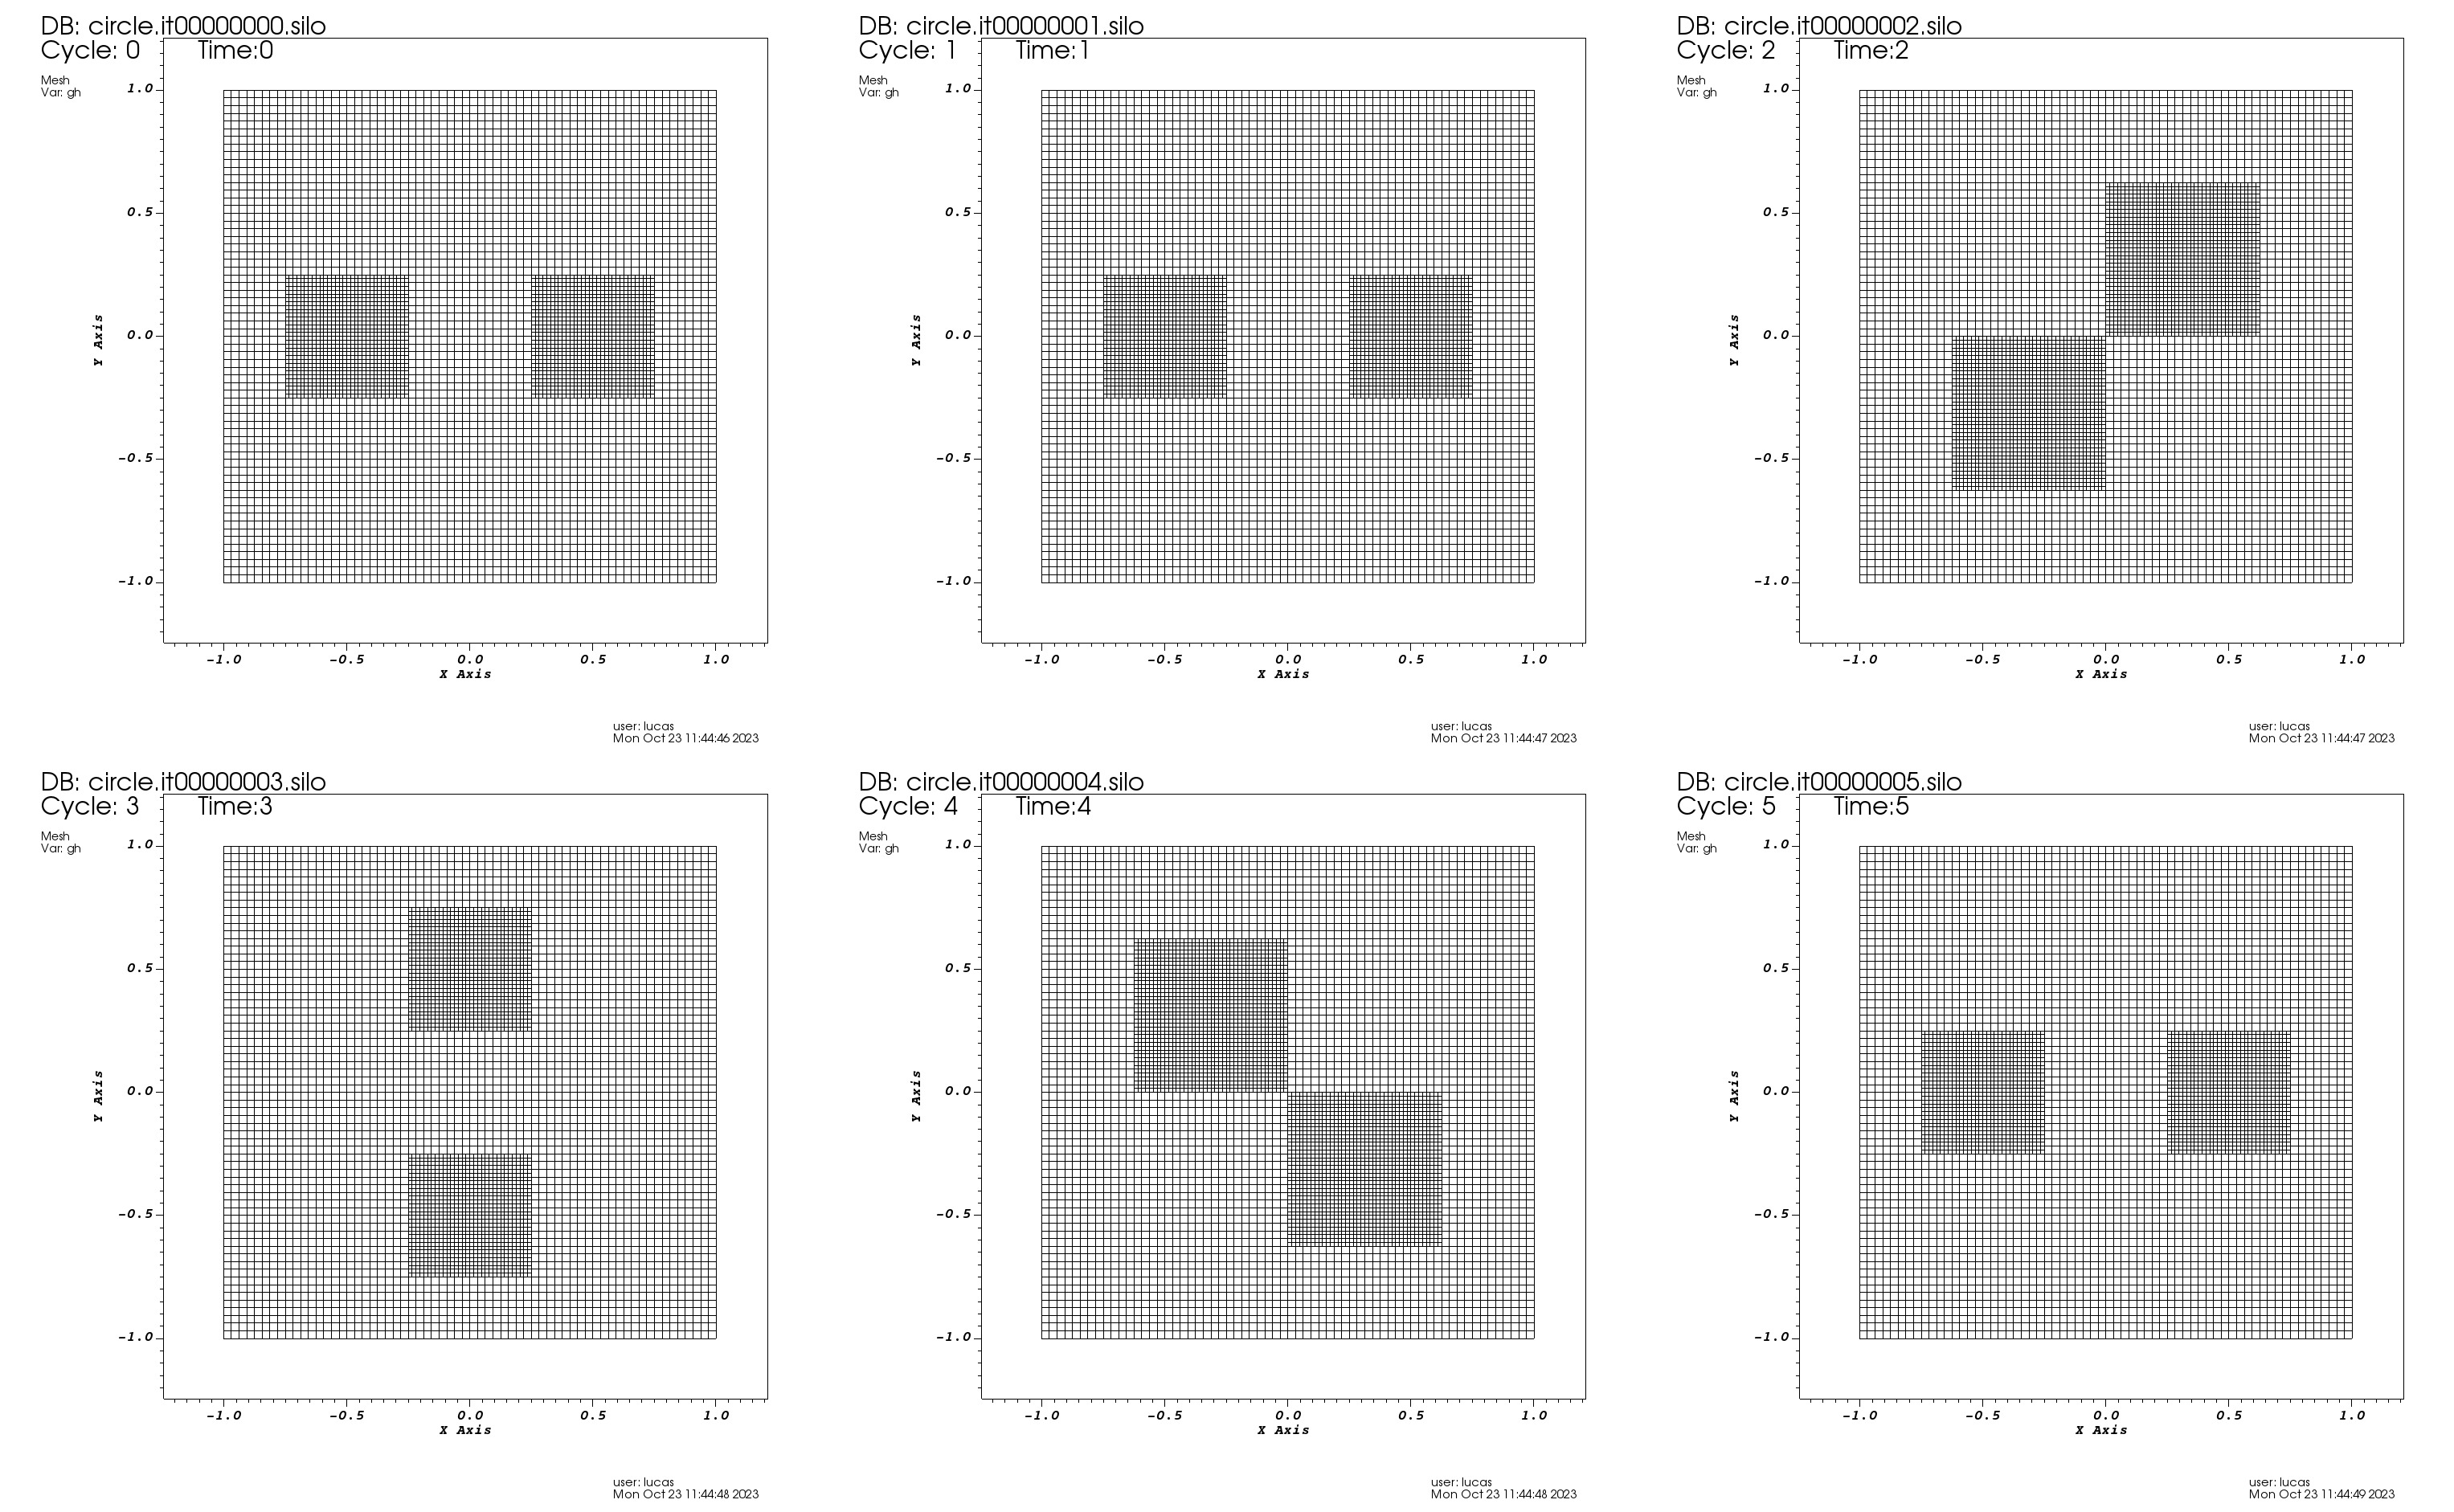
\includegraphics[width=\linewidth]{boxes_frames.png}
  \end{center}
  \caption{AMR boxes moving around a circle, as implemented in the \texttt{MovingBoxToy} thorn.}
  \label{fig:boxes_circle}
\end{figure*}

\subsection{Advanced AMR}
\label{sec:advanced_amr}

\CarpetX\space supports non-fixed (adaptive) mesh refinement. For cell level control of AMR, \CarpetX\space provides user with a cell centered and non-checkpointed grid function called \texttt{regrid\_error}. Users are responsible for filling this grid function with real value however they see fit. Once it is filled, the configuration parameter \texttt{CarpetX::regrid\_error\_threshold} controls regridding: If the values stored in \texttt{regrid\_error} are larger than what is set in \texttt{regrid\_error\_threshold}, the region gets refined. Additionally, the configuration parameter \texttt{CarpetX::regrid\_every} controls how many iterations should pass before checking if the error threshold has been exceeded. The parameter \texttt{CarpetX::max\_num\_levels} controls the maximum number of allowed refinement levels.

Note that \CarpetX\space \textbf{does not} provide a ``standardized'' regrid error routine. This is because refinement criteria are highly specific to the problem being solved via AMR, and thus there is no one size fits all error criteria. This might seem inconvenient, but ultimately it allows for users to have higher degrees of customization in their AMR codes. For demonstration purposes, we shall now provide a routine that estimates the regrinding error as \todo{what? Provide a good starter example}. This implementation could be used as a starting point for codes that wish to use different error criteria in their AMR grids.

\begin{lstlisting}
  extern "C" void EstimateError(CCTK_ARGUMENTS) {
  DECLARE_CCTK_ARGUMENTSX_EstimateError;
  DECLARE_CCTK_PARAMETERS;

  // The template indices indicate this a loop over cell centers
  // Remember that regrid_error is a cell centered grid function
  grid.loop_int_device<1, 1, 1>(
      grid.nghostzones,
      [=] (const Loop::PointDesc &p) {
        // TODO: Give a simple example
        regrid_error(p.I) = 0.0;
      });
}
\end{lstlisting}

Once defined, \texttt{EstimateError} should be scheduled in both the \texttt{postinitial} and \texttt{poststep} bins. The \texttt{poststep} bin gets called right after a new state vector has been calculated, and is thus the proper place to analyze it. The \texttt{postinitial} scheduling is also necessary for computing the initial refinement after initial conditions have been set up. A thorn making use of the \texttt{regrid\_error} AMR mechanism should then add the following to its \texttt{schedule.ccl} file:

\begin{lstlisting}[language=bash]
  SCHEDULE EstimateError AT postinitial
  {
    LANG: C
    READS: state(everywhere)
    WRITES: CarpetX::regrid_error(interior)
  } "Estimate error for regridding"
  
  SCHEDULE EstimateError AT poststep
  {
    LANG: C
    READS: state(everywhere)
    WRITES: CarpetX::regrid_error(interior)
  } "Estimate error for regridding"
\end{lstlisting}

\subsection{Controlling prolongation}

Prolongation refers to the interpolation of data on coarse grid into a finer grid. \CarpetX\space allows users to control how this propagation of data will be executed via the parameter \texttt{CarpetX::prolongation\_type}, whose possible values are detailed in Tab.~\ref{tab:prolongation_methods}. Additionally, other aspects of the prolongation operator can be controlled with the parameters detailed in Tab.~\ref{tab:other_prolongation_params}

\begin{table}[ht]
  \centering
  \begin{tabularx}{\textwidth}{lX}
    Method                   & Description                                                                                                                                   \\\hline\hline
    \texttt{"interpolate"}   & Interpolate between data points                                                                                                               \\
    \texttt{"conservative"}  & Interpolate cell averages, ensuring conservation                                                                                              \\
    \texttt{"ddf"}           & Interpolate in vertex centered and conserve in cell centered directions                                                                       \\
    \texttt{"ddf-eno"}       & Interpolate in vertex centered and ENO-conserve in cell centered directions                                                                   \\
    \texttt{"ddf-hermite"}   & Hermite-interpolate in vertex centered and conserve in cell centered directions                                                               \\
    \texttt{"natural"}       & Interpolate in vertex centered and conserve in cell centered directions, using the same order                                                 \\
    \texttt{"poly-cons3lfb"} & Interpolate polynomially in vertex centered directions and conserve with 3rd order accuracy and a linear fallback in cell centered directions \\\hline\hline
  \end{tabularx}
  \caption{Prolongation methods available in \CarpetX.}
  \label{tab:prolongation_methods}
\end{table}

\begin{table}[ht]
  \centering
  \begin{tabularx}{\textwidth}{lccX}
    Parameter                       & Type                  & Default value & Description                                             \\\hline\hline
    \texttt{prolongation\_order}    & Integer larger than 0 & 1             & Controls the order of the interpolation in prolongation \\
    \texttt{do\_restrict}           & Boolean               & yes           & Automatically restrict fine to coarse grid functions    \\
    \texttt{restrict\_during\_sync} & Boolean               & yes           & Restrict fine to coarse grid functions when syncing     \\
  \end{tabularx}
  \caption{Parameters controlling prolongation in \CarpetX.}
  \label{tab:other_prolongation_params}
\end{table}

%%%%%%%%%%%%%%%%%%%%%%%%%%%%%%%%%%%%%%%%%%%%%%%%%%%%%%%%%%%%
\section{Boundary conditions and symmetries}
\label{sec:bcs}

\CarpetX\space provides a way of setting up standard boundary conditions and symmetry conditions (to be applied on grid boundaries) via parameter files and grid function tags. More complex boundary conditions can be implemented by users but doing so is not often an easy task due to how \texttt{AMReX} works internally.

\subsection{Boundary conditions via parameters}

The following boundary condition types can be specified:

\begin{enumerate}
    \item \texttt{"none"}: Don't apply any boundary condition to the grid. This is the default setting for all boundaries.
    \item \texttt{"dirichlet"}: Dirichlet boundary conditions.
    \item \texttt{"linear extrapolation"}: Linearly extrapolate interior values to boundary values.
    \item \texttt{"neumann"}: Neumann boundary conditions.
    \item \texttt{"robin"}: Robin boundary conditions.
\end{enumerate}

Remember that, given a function $f(x,y,z)$ that satisfies a given PDE in a domain $\Omega \subset \mathbb{R}^n$ whose boundary is denoted by $\partial\Omega$, a Dirichlet boundary condition imposes that
%
\begin{equation}
  f(x,y,z) = g \quad \forall (x,y,z) \in \partial \Omega,
  \label{eq:dirichlet}
\end{equation}
%
a Neumann boundary condition imposes that
%
\begin{equation}
  \frac{\partial f}{\partial \mathbf{n}} = g \quad \forall (x,y,z) \in \partial \Omega,
  \label{eq:neumann}
\end{equation}
%
where $\mathbf{n}$ is the normal to the boundary $\partial \Omega$ and a Robin boundary condition imposes that
%
\begin{equation}
  a f + b \frac{\partial f}{\partial \mathbf{n}} = g \quad \forall (x,y,z) \in \partial \Omega.
  \label{eq:robin}
\end{equation}

The type of boundary condition in all 6 grid faces can be configured independently via the parameters described in Tab.~\ref{tab:boundary_settings}.

\begin{table}[ht]
    \centering
    \begin{tabular}{cc}
    Parameter                   & Description                             \\\hline\hline
    \texttt{boundary\_x}        & Boundary condition at lower $x$ boundary\\
    \texttt{boundary\_upper\_x} & Boundary condition at upper $x$ boundary\\
    \texttt{boundary\_y}        & Boundary condition at lower $y$ boundary\\
    \texttt{boundary\_upper\_y} & Boundary condition at upper $y$ boundary\\
    \texttt{boundary\_z}        & Boundary condition at lower $z$ boundary\\
    \texttt{boundary\_upper\_z} & Boundary condition at upper $z$ boundary\\\hline\hline
    \end{tabular}
    \caption{Parameters controlling boundary condition types in \CarpetX.}
    \label{tab:boundary_settings}
\end{table}

  Once boundary types are chosen, they are applied to all grid functions. Users may override the global configuration for a specific set of grid function in which different boundary conditions should be applied to. This is done by passing a list of space (or new line) separated strings to the appropriate parameter, depending on which boundary condition(s) should be overridden. These parameters are of the form
%
  \begin{center}
    \texttt{CarpetX::<boundary condition name>\_<direction>\_vars = "..."}
  \end{center}
%
where \texttt{<boundary condition name>} is one of
%
\begin{itemize}
  \item \texttt{dirichlet}
  \item \texttt{linear\_extrapolation}
  \item \texttt{neumann}
  \item \texttt{robin}
\end{itemize}
%
and \texttt{<direction>} is one of
\begin{itemize}
  \item \texttt{x}
  \item \texttt{y}
  \item \texttt{z}
  \item \texttt{upper\_x}
  \item \texttt{upper\_y}
  \item \texttt{upper\_z}
\end{itemize}

In order to set the actual values of Dirichlet, Neumann and Robin boundary conditions, users can specify values via the \texttt{TAGS} mechanism in \texttt{interface.ccl}, detailed in Sec.~\ref{sec:tags}. Note that it is only possible to set the quantity $g$ in Eqs~\eqref{eq:dirichlet}-\eqref{eq:robin}. The syntax is as follows

\begin{lstlisting}[language=bash]
  # For Dirichlet BCs
  CCTK_<type> <group-name> TAGS='dirichlet_values={1.0}'
  {
    ...
  } "A group of variables"

  # For Neumman BCs
  CCTK_<type> <group-name> TAGS='neumann_values={1.0}'
  {
    ...
  } "A group of variables"

  # For Robin BCs
  CCTK_<type> <group-name> TAGS='robin_values={1.0}'
  {
    ...
  } "A group of variables"
\end{lstlisting}

If a variable group contains multiple variables or multiple boundary conditions, simply append the boundary values to the brace enclose list of boundary values and add another boundary condition as a tag. For example, consider the 3-metric variable group declared in the \texttt{ADMBaseX} thorn bundled with \CarpetX, which consists of 6 grid functions each with their own Dirichlet and Robin boundary condition values:

\begin{lstlisting}[language=bash]
  CCTK_REAL metric TYPE=gf TAGS='dirichlet_values={1.0 0.0 0.0   1.0 0.0   1.0} robin_values={1.0 0.0 0.0   1.0 0.0   1.0} ...'
  {
    gxx gxy gxz gyy gyz gzz
  } "ADM 3-metric g_ij"
\end{lstlisting}

%%%%%%%%%%%%%%%%%%%%%%%%%%%%%%%%%%%%%%%%%%%%%%%%%%%%%%%%%%%%
\subsection{Symmetry boundary conditions}

\CarpetX\space supports two types of symmetry boundary conditions: Reflections and periodicity. Each of these conditions can be set individually for each grid face as with boundary conditions. To Set reflective symmetry conditions, the parameters in Tab.~\ref{tab:reflection_params} are available. To set periodicity, the parameters in Tab.~\ref{tab:periodic_params} are provided.

\begin{table}[ht]
  \centering
  \begin{tabular}{cc}
  Parameter                     & Description                             \\\hline\hline
  \texttt{reflection\_x}        & Reflection symmetry at lower $x$ boundary\\
  \texttt{reflection\_upper\_x} & Reflection symmetry at upper $x$ boundary\\
  \texttt{reflection\_y}        & Reflection symmetry at lower $y$ boundary\\
  \texttt{reflection\_upper\_y} & Reflection symmetry at upper $y$ boundary\\
  \texttt{reflection\_z}        & Reflection symmetry at lower $z$ boundary\\
  \texttt{reflection\_upper\_z} & Reflection symmetry at upper $z$ boundary\\\hline\hline
  \end{tabular}
  \caption{Parameters controlling reflection symmetry in \CarpetX.}
  \label{tab:reflection_params}
\end{table}

\begin{table}[ht]
  \centering
  \begin{tabular}{cc}
  Parameter            & Description          \\\hline\hline
  \texttt{periodic\_x} & Periodic $x$ boundary\\
  \texttt{periodic\_x} & periodic $y$ boundary\\
  \texttt{periodic\_y} & Periodic $z$ boundary\\\hline\hline
  \end{tabular}
  \caption{Parameters controlling periodicity in \CarpetX.}
  \label{tab:periodic_params}
\end{table}

%%%%%%%%%%%%%%%%%%%%%%%%%%%%%%%%%%%%%%%%%%%%%%%%%%%%%%%%%%%%
\subsection{Custom boundary conditions}

The recommended way of applying custom boundary conditions is to write them to the RHS of the evolution system. Let us once again consider the function that computes the RHS of Eqs.~\eqref{eq:toy_loop_0}-\eqref{eq:toy_loop_1} presented in Sec.~\ref{sec:loops} modified to compute boundary conditions:

\begin{lstlisting}
extern "C" void LoopExample_RHS(CCTK_ARGUMENTS) {
  DECLARE_CCTK_ARGUMENTS_LoopExample_RHS;
  DECLARE_CCTK_PARAMETERS;

  // The grid variable is implicitly defined via the CCTK macros
  // A 0/1 in template parameters indicate that a grid is vertex/cell centered
  grid.loop_int<0, 0, 0>(
    grid.nghostzones,

    // The loop lambda
    [=] (const Loop::PointDesc &p) {
      using std::pow;

      // Instead of computing values for each direction expression
      // explicitly we will use a loop to save us from some typing
      // ddu will store the partial results for each direction
      Arith::vect<CCTK_REAL, dim> ddu;
      
      // Loop over directions
      for (int d = 0; d < dim; ++d) {
        
        // Boundary associated with xmin ymin and zmin
        if (p.BI[d] < 0) {
          ddu[d] = 0;
        }
        // Boundary associated with xmax ymax and zmax
        else if (p.BI[d] > 0) {
          ddu[d] = 0;
        }
        // interior
        else {
          ddu[d] = (u(p.I - p.DI[d]) - 2 * u(p.I) + u(p.I + p.DI[d])) /
                    pow(p.DX[d], 2);
        }
      }

      u_rhs(p.I) = rho(p.I);
      rho_rhs(p.I) = ddu[0] + ddu[1] + ddu[2];

    } // Ending of the loop lambda
  ); // Ending of the loop_int call
}
\end{lstlisting}

Instead of computing derivatives and boundaries for each direction explicitly, we use a loop over each direction, written on line 20. The \texttt{if} branches on lines 23-25 and 27-29 set the values of the RHS of the system in the boundaries associated with the \texttt{xyz\_min} values and \texttt{xyz\_max} values, respectively. In these case, we are setting boundary values to $0$, but users would use whatever boundary condition they require. The takeaway message of this example is to note how one can \textit{access} boundary points, instead of what to write to those points.

%%%%%%%%%%%%%%%%%%%%%%%%%%%%%%%%%%%%%%%%%%%%%%%%%%%%%%%%%%%%
\section{Interpolation}
\label{sec:interpolation}

The recommended way of performing interpolation is using the flesh interface for interpolation by calling \texttt{CCTK\_InterpGridArrays()}, as documented on Sec.~C1.7.4 of the \Cactus\space user guide and with detailed API description in Sec.~A149 of the \Cactus\space reference manual.

Internally, this functionality is implemented by the \texttt{DriverInterpolate} function. If users desire, they can call it directly instead of using \texttt{CCTK\_InterpGridArrays()}. In order to do so, users must add the following to their \texttt{interface.ccl} file
%
\begin{lstlisting}[language=bash]
  CCTK_INT FUNCTION DriverInterpolate(
    CCTK_POINTER_TO_CONST IN cctkGH,
    CCTK_INT IN N_dims,
    CCTK_INT IN local_interp_handle,
    CCTK_INT IN param_table_handle,
    CCTK_INT IN coord_system_handle,
    CCTK_INT IN N_interp_points,
    CCTK_INT IN interp_coords_type,
    CCTK_POINTER_TO_CONST ARRAY IN interp_coords,
    CCTK_INT IN N_input_arrays,
    CCTK_INT ARRAY IN input_array_indices,
    CCTK_INT IN N_output_arrays,
    CCTK_INT ARRAY IN output_array_types,
    CCTK_POINTER ARRAY IN output_arrays)
  REQUIRES FUNCTION DriverInterpolate
\end{lstlisting}

Note that \texttt{DriverInterpolate} and \texttt{CCTK\_InterpGridArrays()} receive exactly the same arguments (again, a complete description of these is given in Sec.~A149 of the \Cactus\space reference manual) but some arguments are unused by \CarpetX. These are \texttt{coord\_system\_handle}, \texttt{interp\_coords\_type\_code}, \texttt{output\_array\_type\_codes} and \texttt{interp\_handle}. Here's and example of a \texttt{DriverInterpolate} call where these ignored parameters are set to zero:

\begin{lstlisting}
  // DriverInterpolate arguments that aren't currently used
  CCTK_INT const coord_system_handle = 0;
  CCTK_INT const interp_coords_type_code = 0;
  CCTK_INT const output_array_type_codes[1] = {0};
  int interp_handle = 0;

  // We assume that the other (non-ignored) parameters exist
  // within the scope but are ommited from this snippet for clarity
  DriverInterpolate(
      cctkGH, N_dims, interp_handle, param_table_handle, coord_system_handle,
      npoints, interp_coords_type_code, interp_coords, nvars, (int const*const)varinds,
      nvars, output_array_type_codes, output_array);
\end{lstlisting}

Lastly, to control the order of the interpolation operators, users can set the \texttt{CarpetX::interpolation\_order} parameter, which defaults to 1 and must be greater than 0.

%%%%%%%%%%%%%%%%%%%%%%%%%%%%%%%%%%%%%%%%%%%%%%%%%%%%%%%%%%%%
\section{Performance tuning}
\label{sec:perf_tuning}

\subsection{Parallelism model}

When running on CPUs, \AMReX\space will divide the grid in boxes whose sizes are controlled by \texttt{blocking\_factor} and \texttt{max\_grid\_size} parameter families. These will be distributed over MPI ranks and each rank will subdivide the boxes on \textit{tiles}. This subdivision into tiles is only logical (not in memory). Threads may then process tiles in any random order. When running on GPU's, tiling is disabled and \AMReX\space tries to assign one GPU per MPI process. If there are more MPI processes than grids to distribute, some MPI process may become idle. To prevent this from happening, the \texttt{CarpetX::refine\_grid\_layout} (see bellow) can be used to ensure that each MPI rank processes at least one grid.

\subsection{Parallelism control parameters}

\CarpetX\space allows users to control \texttt{AMReX}'s underlying load balancing mechanism by exposing \texttt{AMReX} parameters to \texttt{Cactus} parameter files. We shall now describe these parameters and their functionality.

\subsubsection{\texttt{CarpetX::max\_grid\_size\_\{xyz\}}}

\AMReX\space will divide the domain in every direction so that each grid is no longer than \texttt{max\_grid\_size} in that direction. It defaults to 32 in each coordinate direction.

\subsubsection{\texttt{CarpetX::blocking\_factor\_\{xyz\}}}

Constrain grid creation so that each grid must be divisible by \texttt{blocking\_factor}. This implies that both the domain (at each level) and \texttt{max\_grid\_size} must be divisible by \texttt{blocking\_factor}, and that \texttt{blocking\_factor} must be either 1 or a power of 2. It defaults to 8 in every direction.

\subsubsection{\texttt{CarpetX::refine\_grid\_layout}}

If set to \texttt{"yes"} and the number of grids created is less than the number of processors ($N_\text{grids} < N_\text{procs}$), then grids will be further subdivided until $N_\text{grids} \geq N_\text{procs}$. If subdividing the grids to achieve $N_\text{grids} \geq N_\text{procs}$ would violate the \texttt{blocking\_factor} criterion then additional grids are not created and the number of grids will remain less than the number of processors. It defaults to \texttt{"yes"}

\subsubsection{\texttt{CarpetX::grid\_efficiency}}

Because mesh refinement in \AMReX is done per-cell (see sec.~\ref{sec:advanced_amr} for further details), a refinement region may be irregular. \AMReX\space can only deal with logically cubical grids, thus a refinement region will be replaced by a new grid consisting of coarse and finer boxes on the region. Due to this ``discretization'' of the refinement region, more cells will be refined than necessary. Refining too many points becomes obviously inefficient. Conversely, refining too few points is also non-ideal, as it leads to a grid structure consisting of many small boxes. ``Grid efficiency'' then refers to the ratio of the points that need to be refined over the points that actually are refined in the new grid structure. This steers AMReX's eagerness to combine smaller boxes into larger ones by refining more points. The default value for this parameter is $0.7$

\subsubsection{\texttt{CarpetX::max\_tile\_size\_\{xyz\}}}

Controls tile sizes. In order to be cache efficient, tiling is disabled in the \texttt{x} direction because these elements are not stored contiguously in memory. The default values for \texttt{max\_tile\_size} are given in Tab.~\ref{tab:tile_sizes}. These default values were found trough experimentation. Users are encouraged to change them in order to achieve optimal performance in their machines and use cases.

\begin{table}[h]
  \centering
  \begin{tabular}{cc}
    Parameter                   & Default value        \\\hline\hline
    \texttt{max\_tile\_size\_x} & $1024000$ (disabled) \\
    \texttt{max\_tile\_size\_y} & $16$                 \\
    \texttt{max\_tile\_size\_z} & $32$                 \\\hline\hline
  \end{tabular}
  \caption{\CarpetX's tile size control parameters and their default values.}
  \label{tab:tile_sizes}
\end{table}


%%%%%%%%%%%%%%%%%%%%%%%%%%%%%%%%%%%%%%%%%%%%%%%%%%%%%%%%%%%%
\section{Profiling}
\label{sec:profiling}

Profiling refers to the act of collecting runtime and other performance data on the execution of an application in order to improve its performance characteristics. The recommended way of profiling \CarpetX\space applications is using \href{http://hpctoolkit.org/}{\texttt{HPCToolkit}}. We recommend that user first read the software's \href{http://hpctoolkit.org/manual/HPCToolkit-users-manual.pdf}{documentation} thoroughly. 

Installing \texttt{HPCToolkit} on an HPC system will probably require the help of the system's administrators. Once installed, the application should be launched with the \texttt{hpcrun} command, which will automatically collect performance data from the launched application. To profile \CarpetX\space while using an HPC system, the recommended steps are:
%
\begin{enumerate}
  \item Launch an interactive section with the cluster's job system. In this session, the \texttt{mpirun} and \texttt{hpcrun} commands should be available.
  
  \item Navigate to the directory where the \Cactus\space executable is located. Given a configuration named \texttt{config-name}, the executable is located in \texttt{Cactus/exe/cactus\_config-name}.
  
  \item Select a parameter file to execute and gather performance information on. Let us call it \texttt{perf.par} and suppose that it is located in \texttt{Cactus/exe/}.
  
  \item Assuming that the system's \texttt{MPI} launcher is called \texttt{mpirun}, to profile a CPU application, issue
  %
  \begin{lstlisting}[language=bash]
    mpirun hpcrun ./cactus_config-name perf.par
  \end{lstlisting}
  %
  To profile a GPU application, issue
  %
  \begin{lstlisting}[language=bash]
    mpirun hpcrun -e gpu=<vendor> ./cactus_config-name perf.par
  \end{lstlisting}
  %
  where \texttt{<vendor>} is either \texttt{nvidia} or \texttt{amd}, depending on which GPU chips are available in the system.

  \item After \Cactus\space completes the evolution, a new folder called \texttt{hpctoolkit-cactus\_config-name-measurements} will be created on the same directory where \texttt{hpcrun} was executed. \texttt{HPCToolkit} needs to recover program structure in order to create better profiling information. To do that, issue
  %
  \begin{lstlisting}[language=bash]
    hpcstruct hpctoolkit-cactus_config-name-measurements
  \end{lstlisting}

  \item Finally, to have \texttt{HPCToolkit} analyze measurements and attribute it to source code, issue
  %
  \begin{lstlisting}[language=bash]
    hpcprof hpctoolkit-cactus_config-name-measurements
  \end{lstlisting}
\end{enumerate}

This will generate the \texttt{hpctoolkit-cactus\_config-name-database} folder, which can be used with \texttt{HPCToolkit}'s provided profile visualization tool called \href{http://hpctoolkit.org/download.html}{\texttt{hpcviewer}}. See chapter 10 of the \texttt{HPCToolkit} \href{http://hpctoolkit.org/manual/HPCToolkit-users-manual.pdf}{manual} for usage details.

%%%%%%%%%%%%%%%%%%%%%%%%%%%%%%%%%%%%%%%%%%%%%%%%%%%%%%%%%%%%
\section{Outputting data}
\label{sec:data}

\CarpetX\space outputs data in the following formats: \texttt{Silo}, \texttt{openPMD} (with various backends), \texttt{Adios2} and \texttt{TSV}. For each output format, users can choose what and how frequently variables will be written to disk. In the following sections we will provide details to each format.

\subsection{TSV}
\label{sec:tsv}

The \texttt{TSV} acronym stands for Tab Separated Values. This is a plain text format in which data is written to files in rows (lines) and columns, each column separated by a tab character. These formats are very easy to hand parse and manipulate or post-process. Many open source tools are also available for reading this format out of the box (see for instance the \texttt{Python} framework \texttt{Pandas}). There are however two important disadvantages in using plain text formats: The first is a loss of precision when converting floating point numbers from binary to string representation and converting from string back into binary form, due to the way floating point numbers work. The second is compactness. While a 16 digit double precision floating point number takes 8 bytes to be represented in binary form, it requires at least 17 bytes (1 byte per digit plus the floating point dot) to be represented as a string. For these reasons, this format is not recommended to production runs or to complex data analysis. It is useful however, for quick and easy visualizations or diagnostics of data. It is also useful when other, more sophisticated formats are not available.

To control \texttt{TSV} output, \CarpetX\space provides the parameters described in Tab.~\ref{tab:tsv_params}

\begin{table}[ht]
  \centering
  \begin{tabularx}{\textwidth}{cccX}
    Parameter                & Type    & Default Value  & Description \\\hline\hline
    \texttt{out\_tsv}        & Boolean & \texttt{"yes"} & Whether to produce \texttt{TSV} output \\
    \texttt{out\_tsv\_vars}  & String  & Empty string   & Space or newline separated string of grid functions to output \\
    \texttt{out\_tsv\_every} & Integer & $-1$           & If set to $-1$, output is produced as often as the setting of \texttt{IO::out\_every}. If set to $0$, output is never produced. If set to $1$ or larger, output every that many iterations \\\hline\hline
  \end{tabularx}
  \label{tab:tsv_params}
  \caption{\CarpetX\space parameters for \texttt{TSV} output.}
\end{table}

As an example, to output the grid functions of \texttt{WaveToyX} as \texttt{TSV} files every 2 iterations, one would write in their parameter file the following excerpt

\begin{lstlisting}[language=bash]
  CarpetX::out_tsv = yes
  CarpetX::out_tsv_every = 2
  CarpetX::out_tsv_vars = "
    WaveToyX::state
    WaveToyX::rhs
    WaveToyX::energy
    WaveToyX::error
"
\end{lstlisting}

\subsection{SILO}
\label{sec:silo}

The \texttt{Silo} format (see \href{https://visit-sphinx-github-user-manual.readthedocs.io/en/develop/data_into_visit/SiloFormat.html}{here} for more information) is the native file format of the \href{https://sd.llnl.gov/simulation/computer-codes/visit}{VisIt} data visualization tool. Given its native support in \texttt{VisIt}, \texttt{silo} files are good for direct visualization of simulation data and grids (Fig.~\ref{fig:boxes_circle} of this document as well as the \texttt{animated\_boxes.gif} file in the documentation folder were both created with \texttt{VisIt}).

To control \texttt{SILO} output, \CarpetX\space provides the parameters described in Tab.~\ref{tab:silo_params}

\begin{table}[ht]
  \centering
  \begin{tabularx}{\textwidth}{cccX}
    Parameter                 & Type    & Default Value  & Description \\\hline\hline
    \texttt{out\_silo\_vars}  & String  & Empty string   & Space or newline separated string of grid functions to output \\
    \texttt{out\_silo\_every} & Integer & $-1$           & If set to $-1$, output is produced as often as the setting of \texttt{IO::out\_every}. If set to $0$, output is never produced. If set to $1$ or larger, output every that many iterations \\\hline\hline
  \end{tabularx}
  \label{tab:silo_params}
  \caption{\CarpetX\space parameters for \texttt{SILO} output.}
\end{table}

As an example, to output the grid functions of \texttt{WaveToyX} as \texttt{SILO} files every 2 iterations, one would write in their parameter file the following excerpt

\begin{lstlisting}[language=bash]
  CarpetX::out_silo_every = 2
  CarpetX::out_silo_vars = "
    WaveToyX::state
    WaveToyX::rhs
    WaveToyX::energy
    WaveToyX::error
"
\end{lstlisting}

\subsection{openPMD}
\label{sec:openpmd}

\texttt{openPMD} stands for ``open standard for particle-mesh data files''. Strictly speaking, it is not a file format, but a standard for meta-data, naming schemes and file organization. \texttt{openPMD} is thus ``backed'' by usual hierarchical binary data formats, such as \texttt{HDF5} and \texttt{Adios2}, both supported by \CarpetX. Put simply, \texttt{openPMD} specifies a standardized and interchangeable way of organizing data within \texttt{HDF5} and \texttt{Adios2} files.

To control \texttt{openPMD} output, \CarpetX\space provides the parameters described in Tab.~\ref{tab:openpmd_params}

\begin{table}[ht]
  \centering
  \begin{tabularx}{\textwidth}{cccX}
    Parameter                 & Type    & Default Value  & Description \\\hline\hline
    \texttt{out\_openpmd\_vars}  & String  & Empty string   & Space or newline separated string of grid functions to output \\
    \texttt{out\_openpmd\_every} & Integer & $-1$           & If set to $-1$, output is produced as often as the setting of \texttt{IO::out\_every}. If set to $0$, output is never produced. If set to $1$ or larger, output every that many iterations \\\hline\hline
  \end{tabularx}
  \label{tab:openpmd_params}
  \caption{\CarpetX\space parameters for \texttt{SILO} output.}
\end{table}

Additionally, it is possible to control which ``backing'' format to use with \texttt{openPMD} via the \texttt{CarpetX::openpmd\_format} parameter, whose possible string values are listed in Tab~\ref{tab:openpmd_formats}

\begin{table}[ht]
  \centering
  \begin{tabular}{cc}
    Value         & Description                                                                                                                                                                 \\ \hline\hline
    \texttt{"HDF5"}        & The Hierarchical Data Format, version 5 (see \href{https://www.hdfgroup.org/solutions/hdf5/}{here})                                                                \\
    \texttt{"ADIOS1"}      & The Adaptable I/O System version 1 (see \href{https://csmd.ornl.gov/software/adios-1x}{here})                                                                      \\
    \texttt{"ADIOS2"}      & The Adaptable I/O System version 2 (see \href{https://adios2.readthedocs.io/en/v2.9.2/}{here}). Requires \texttt{openPMD\_api} $< 0.15$                            \\
    \texttt{"ADIOS2\_BP"}  & ADIOS2 native binary-pack. Requires \texttt{openPMD\_api} $\geq0.15$                                                                                                   \\
    \texttt{"ADIOS2\_BP4"} & ADIOS2 native binary-pack version 4 (see \href{https://adios2.readthedocs.io/en/latest/engines/engines.html#bp5}{here}). Requires \texttt{openPMD\_api} $\geq0.15$ \\
    \texttt{"ADIOS2\_BP5"} & ADIOS2 native binary-pack version 5 (see \href{https://adios2.readthedocs.io/en/latest/engines/engines.html#bp5}{here}). Requires \texttt{openPMD\_api} $\geq0.15$ \\
    \texttt{"ADIOS2\_SST"} & ADIOS2 Sustainable Staging Transport (see \href{n ADIOS2, the Sustainable Staging Transport (SST)}{hee})                                                           \\
    \texttt{"ADIOS2\_SSC"} & ADIOS2 Strong Staging Coupler (see \href{Strong Staging Coupler}{here})                                                                                            \\
    \texttt{"JSON"}        & JavaScript Object Notation (see \href{https://www.json.org/json-en.html}{here})                                                                                    \\ \hline\hline
  \end{tabular}
  \label{tab:openpmd_formats}
  \caption{Possible values for \texttt{CarpetX::openpmd\_format} controlling \texttt{openPMD}'s storage format.}
\end{table}

When using \texttt{openPMD} output, \CarpetX\space can produce files that can be visualized with \texttt{VisIt}. To do that for \texttt{WaveToyX}, for example, the following excerpt would be added to a parameter file

\begin{lstlisting}[language=bash]
  # It is very important to produce BP4 files, as BP5
  # cannot be imported into VisIt at the time of writing
  CarpetX::openpmd_format = "ADIOS2_BP4"
  
  CarpetX::out_openpmd_vars = "
      WaveToyX::state
      WaveToyX::rhs
      WaveToyX::energy
      WaveToyX::error
  "
\end{lstlisting}

When loading data into \texttt{VisIt}, users must open the \texttt{*.pmd.visit} file produced together with the simulation output. It is also \textit{imperative} to select the file format as \texttt{ADIOS2} in \texttt{VisIt}'s file selector window, otherwise the files will not be loaded correctly.

In addition to \texttt{VisIt}, users can find in the \texttt{CarpetX/doc/openpmd-plot} folder a sample \texttt{Python} script for extracting and plotting data from \CarpetX\space produced \texttt{openPMD} files. The best way to interact with the script is using a \texttt{Python} virtual environment. First, navigate to the \texttt{CarpetX/doc/openpmd-plot} and issue the following commands:

\begin{lstlisting}[language=bash]
python -m venv venv             # Creates the virtual environment.
source venv/bin/activate        # Activates the virtual environment.
pip install -r requirements.txy # Installs required packages.
python plot-zslice.py -h        # See the options available.
deactivate                      # Exits the environment when done.
\end{lstlisting}

\subsection{Pure \texttt{ADIOS2} files}

To output pure \texttt{ADIOS2 BP5} files, (without \texttt{openPMD} formatting), users can use the parameters described in Tab.~\ref{tab:adios2_params}. Note that this output mode produces \texttt{BP5} files, which cannot be read by \texttt{VisIt} (at the time of writing). Users may have to rely on their own tools and scripts for data processing and visualization.

\begin{table}[ht]
  \centering
  \begin{tabularx}{\textwidth}{cccX}
    Parameter                 & Type    & Default Value  & Description \\\hline\hline
    \texttt{out\_adios2\_vars}  & String  & Empty string   & Space or newline separated string of grid functions to output \\
    \texttt{out\_adios2\_every} & Integer & $-1$           & If set to $-1$, output is produced as often as the setting of \texttt{IO::out\_every}. If set to $0$, output is never produced. If set to $1$ or larger, output every that many iterations \\\hline\hline
  \end{tabularx}
  \label{tab:adios2_params}
  \caption{\CarpetX\space parameters for \texttt{ADIOS2} output.}
\end{table}

As an example, to produce \texttt{ADIOS2} files at every $2$ time steps in \texttt{WaveToyX}, users would use the following excerpt

\begin{lstlisting}[language=bash]
  CarpetX::out_adios2_every = 2
  CarpetX::out_adios2_vars = "
    WaveToyX::state
    WaveToyX::rhs
    WaveToyX::energy
    WaveToyX::error
"
\end{lstlisting}

\subsection{Norms files}

\CarpetX can output various norms of grid functions, such as min., max., L2 and others. This output works similarly to the previously described methods. To control norm output, the parameters in Tab.~\ref{tab:norms_output} are provided.

\begin{table}[hb]
  \centering
  \begin{tabularx}{\textwidth}{cccX}
    Parameter                 & Type    & Default Value  & Description \\\hline\hline
    \texttt{out\_norm\_vars}  & String  & Empty string   & Space or newline separated string of grid functions to output \\
    \texttt{out\_norm\_every} & Integer & $-1$           & If set to $-1$, output is produced as often as the setting of \texttt{IO::out\_every}. If set to $0$, output is never produced. If set to $1$ or larger, output every that many iterations \\\hline\hline
  \end{tabularx}
  \label{tab:norms_output}
  \caption{\CarpetX\space parameters for norms output.}
\end{table}

For example, to output \texttt{openPMD} and norms for the \texttt{WaveToyX} thorn grid functions, the following excerpt could be added to a parameter file

\begin{lstlisting}[language=bash]
  CarpetX::out_norm_every = 2
  
  # Here we choose to output only norms of the error grid function    
  CarpetX::out_norm_vars = "
      WaveToyX::error
  "

  # It is very important to produce BP4 files, as BP5
  # cannot be imported into VisIt at the time of writing
  CarpetX::openpmd_format = "ADIOS2_BP4"
  
  CarpetX::out_openpmd_vars = "
      WaveToyX::state
      WaveToyX::rhs
      WaveToyX::energy
      WaveToyX::error
  "
\end{lstlisting}

\subsection{Performance file}

\CarpetX\space can produce a file called \texttt{performance.yaml} with various performance timers for certain iterations of a simulation. This output mirrors that of \texttt{stdout} and may be useful for thorn developers while benchmarking their codes. Controlling performance output is done similarly as to other types of output. The parameters for controlling it are detailed in Tab~\ref{tab:perf_output}

\begin{table}[ht]
  \centering
  \begin{tabularx}{\textwidth}{cccX}
    Parameter                       & Type     & Default Value  & Description \\\hline\hline
    \texttt{out\_performance}        & Boolean & \texttt{"yes"} & Whether to produce performance data in YAML format. \\
    \texttt{out\_performance\_every} & Integer & $-1$           & If set to $-1$, output is produced as often as the setting of \texttt{IO::out\_every}. If set to $0$, output is never produced. If set to $1$ or larger, output every that many iterations. \\\hline\hline
  \end{tabularx}
  \label{tab:perf_output}
  \caption{\CarpetX\space parameters for performance output.}
\end{table}

As an example, to  have performance measurements output for a simulation every 2 iterations, the following parameters may be added to a parameter file

\begin{lstlisting}[language=bash]
  CarpetX::out_performance = yes  
  CarpetX::out_performance_every = 2
\end{lstlisting}

%%%%%%%%%%%%%%%%%%%%%%%%%%%%%%%%%%%%%%%%%%%%%%%%%%%%%%%%%%%%
\section{Debugging}
\label{sec:debugging}

To debug \CarpetX\space applications, users have access to the following parameters: 
%
\begin{itemize}
    \item \texttt{verbose}: A boolean parameter that controls weather or not \CarpetX\space produces verbose output. This output details more of what the driver is doing internally, aiding users in finding bugs. Its default value is \texttt{no}.

    \item \texttt{poison\_undefined\_values}: Sets undefined grid point values to \texttt{NaN} (not a number). By visualizing locations where grid functions contain \texttt{NaN}s, users can determine which grid points are not being filled correctly. Its default value is \texttt{yes}.
\end{itemize}

%%%%%%%%%%%%%%%%%%%%%%%%%%%%%%%%%%%%%%%%%%%%%%%%%%%%%%%%%%%%
%\section{Acknowledgements}

%\begin{thebibliography}{9}
%\end{thebibliography}

% Do not delete next line
% END CACTUS THORNGUIDE

\end{document}
